\documentclass[a4paper,12pt,twoside]{memoir}

% Castellano
\usepackage[spanish,es-tabla]{babel}
\selectlanguage{spanish}
\usepackage[utf8]{inputenc}
\usepackage[T1]{fontenc}
\usepackage{lmodern} % scalable font
\usepackage{microtype}
\usepackage{placeins}

\RequirePackage{booktabs}
\RequirePackage[table]{xcolor}
\RequirePackage{xtab}
\RequirePackage{multirow}

%Extras
\usepackage{tabularx}
\usepackage{longtable}
\usepackage{graphicx}
\usepackage{xcolor}

\definecolor{fucsia}{RGB}{255, 0, 255}
\definecolor{flirk}{RGB}{147, 0, 147}
\definecolor{azulWorker}{RGB}{40, 230, 255}
\definecolor{endeavour}{RGB}{0, 81, 164}

% Links
\PassOptionsToPackage{hyphens}{url}\usepackage[colorlinks]{hyperref}
\hypersetup{
	allcolors = {red}
}

% Ecuaciones
\usepackage{amsmath}

% Rutas de fichero / paquete
\newcommand{\ruta}[1]{{\sffamily #1}}

% Párrafos
\nonzeroparskip

% Huérfanas y viudas
\widowpenalty100000
\clubpenalty100000

% Evitar solapes en el header
\nouppercaseheads

% Imagenes
\usepackage{graphicx}
\newcommand{\imagen}[2]{
	\begin{figure}[!h]
		\centering
		\includegraphics[width=0.9\textwidth]{#1}
		\caption{#2}\label{fig:#1}
	\end{figure}
	\FloatBarrier
}

\newcommand{\imagenflotante}[2]{
	\begin{figure}%[!h]
		\centering
		\includegraphics[width=0.9\textwidth]{#1}
		\caption{#2}\label{fig:#1}
	\end{figure}
}



% El comando \figura nos permite insertar figuras comodamente, y utilizando
% siempre el mismo formato. Los parametros son:
% 1 -> Porcentaje del ancho de página que ocupará la figura (de 0 a 1)
% 2 --> Fichero de la imagen
% 3 --> Texto a pie de imagen
% 4 --> Etiqueta (label) para referencias
% 5 --> Opciones que queramos pasarle al \includegraphics
% 6 --> Opciones de posicionamiento a pasarle a \begin{figure}
\newcommand{\figuraConPosicion}[6]{%
  \setlength{\anchoFloat}{#1\textwidth}%
  \addtolength{\anchoFloat}{-4\fboxsep}%
  \setlength{\anchoFigura}{\anchoFloat}%
  \begin{figure}[#6]
    \begin{center}%
      \Ovalbox{%
        \begin{minipage}{\anchoFloat}%
          \begin{center}%
            \includegraphics[width=\anchoFigura,#5]{#2}%
            \caption{#3}%
            \label{#4}%
          \end{center}%
        \end{minipage}
      }%
    \end{center}%
  \end{figure}%
}

%
% Comando para incluir imágenes en formato apaisado (sin marco).
\newcommand{\figuraApaisadaSinMarco}[5]{%
  \begin{figure}%
    \begin{center}%
    \includegraphics[angle=90,height=#1\textheight,#5]{#2}%
    \caption{#3}%
    \label{#4}%
    \end{center}%
  \end{figure}%
}
% Para las tablas
\newcommand{\otoprule}{\midrule [\heavyrulewidth]}
%
% Nuevo comando para tablas pequeñas (menos de una página).
\newcommand{\tablaSmall}[5]{%
 \begin{table}
  \begin{center}
   \rowcolors {2}{gray!35}{}
   \begin{tabular}{#2}
    \toprule
    #4
    \otoprule
    #5
    \bottomrule
   \end{tabular}
   \caption{#1}
   \label{tabla:#3}
  \end{center}
 \end{table}
}

%
%Para el float H de tablaSmallSinColores
\usepackage{float}

%
% Nuevo comando para tablas pequeñas (menos de una página).
\newcommand{\tablaSmallSinColores}[5]{%
 \begin{table}[H]
  \begin{center}
   \begin{tabular}{#2}
    \toprule
    #4
    \otoprule
    #5
    \bottomrule
   \end{tabular}
   \caption{#1}
   \label{tabla:#3}
  \end{center}
 \end{table}
}

\newcommand{\tablaApaisadaSmall}[5]{%
\begin{landscape}
  \begin{table}
   \begin{center}
    \rowcolors {2}{gray!35}{}
    \begin{tabular}{#2}
     \toprule
     #4
     \otoprule
     #5
     \bottomrule
    \end{tabular}
    \caption{#1}
    \label{tabla:#3}
   \end{center}
  \end{table}
\end{landscape}
}

%
% Nuevo comando para tablas grandes con cabecera y filas alternas coloreadas en gris.
\newcommand{\tabla}[6]{%
  \begin{center}
    \tablefirsthead{
      \toprule
      #5
      \otoprule
    }
    \tablehead{
      \multicolumn{#3}{l}{\small\sl continúa desde la página anterior}\\
      \toprule
      #5
      \otoprule
    }
    \tabletail{
      \hline
      \multicolumn{#3}{r}{\small\sl continúa en la página siguiente}\\
    }
    \tablelasttail{
      \hline
    }
    \bottomcaption{#1}
    \rowcolors {2}{gray!35}{}
    \begin{xtabular}{#2}
      #6
      \bottomrule
    \end{xtabular}
    \label{tabla:#4}
  \end{center}
}

%
% Nuevo comando para tablas grandes con cabecera.
\newcommand{\tablaSinColores}[6]{%
  \begin{center}
    \tablefirsthead{
      \toprule
      #5
      \otoprule
    }
    \tablehead{
      \multicolumn{#3}{l}{\small\sl continúa desde la página anterior}\\
      \toprule
      #5
      \otoprule
    }
    \tabletail{
      \hline
      \multicolumn{#3}{r}{\small\sl continúa en la página siguiente}\\
    }
    \tablelasttail{
      \hline
    }
    \bottomcaption{#1}
    \begin{xtabular}{#2}
      #6
      \bottomrule
    \end{xtabular}
    \label{tabla:#4}
  \end{center}
}

%
% Nuevo comando para tablas grandes sin cabecera.
\newcommand{\tablaSinCabecera}[5]{%
  \begin{center}
    \tablefirsthead{
      \toprule
    }
    \tablehead{
      \multicolumn{#3}{l}{\small\sl continúa desde la página anterior}\\
      \hline
    }
    \tabletail{
      \hline
      \multicolumn{#3}{r}{\small\sl continúa en la página siguiente}\\
    }
    \tablelasttail{
      \hline
    }
    \bottomcaption{#1}
  \begin{xtabular}{#2}
    #5
   \bottomrule
  \end{xtabular}
  \label{tabla:#4}
  \end{center}
}



\definecolor{cgoLight}{HTML}{EEEEEE}
\definecolor{cgoExtralight}{HTML}{FFFFFF}

%
% Nuevo comando para tablas grandes sin cabecera.
\newcommand{\tablaSinCabeceraConBandas}[5]{%
  \begin{center}
    \tablefirsthead{
      \toprule
    }
    \tablehead{
      \multicolumn{#3}{l}{\small\sl continúa desde la página anterior}\\
      \hline
    }
    \tabletail{
      \hline
      \multicolumn{#3}{r}{\small\sl continúa en la página siguiente}\\
    }
    \tablelasttail{
      \hline
    }
    \bottomcaption{#1}
    \rowcolors[]{1}{cgoExtralight}{cgoLight}

  \begin{xtabular}{#2}
    #5
   \bottomrule
  \end{xtabular}
  \label{tabla:#4}
  \end{center}
}




\graphicspath{ {./img/} }

% Capítulos
\chapterstyle{bianchi}
\newcommand{\capitulo}[2]{
	\setcounter{chapter}{#1}
	\setcounter{section}{0}
	\setcounter{figure}{0}
	\setcounter{table}{0}
	\chapter*{#2}
	\addcontentsline{toc}{chapter}{#2}
	\markboth{#2}{#2}
}

% Apéndices
\renewcommand{\appendixname}{Apéndice}
\renewcommand*\cftappendixname{\appendixname}

\newcommand{\apendice}[1]{
	%\renewcommand{\thechapter}{A}
	\chapter{#1}
}

\renewcommand*\cftappendixname{\appendixname\ }

% Formato de portada
\makeatletter
\usepackage{xcolor}
\newcommand{\tutor}[1]{\def\@tutor{#1}}
\newcommand{\course}[1]{\def\@course{#1}}
\definecolor{cpardoBox}{HTML}{E6E6FF}
\def\maketitle{
  \null
  \thispagestyle{empty}
  % Cabecera ----------------
\noindent
\includegraphics[width=\textwidth]{cabecera}\vspace{1cm}%
  \vfill
  % Título proyecto y escudo informática ----------------
  \colorbox{cpardoBox}{%
    \begin{minipage}{.8\textwidth}
      \vspace{.5cm}\Large
      \begin{center}
      \textbf{TFG del Grado en Ingeniería Informática}\vspace{.6cm}\\
      \textbf{\LARGE\@title{}}
      \end{center}
      \vspace{.2cm}
    \end{minipage}

  }%
  \hfill\begin{minipage}{.20\textwidth}
    
\includegraphics[width=\textwidth]{escudoInfor}
  \end{minipage}
  \vfill
  % Datos de alumno, curso y tutores ------------------
  \begin{center}%
  {%
    \noindent\LARGE
    Presentado por \@author{}\\ 
    en Universidad de Burgos --- \@date{}\\
    Tutor: \@tutor{}\\
  }%
  \end{center}%
  \null
  \cleardoublepage
  }
\makeatother


% Datos de portada
\title{Desarrollo de un videojuego del género Plataformas 2D en Unity \\Documentación Técnica}
\author{Marcos Romano Ibáñez}
\tutor{Jesús María Alonso Abad}
\date{\today}

\begin{document}

\maketitle



\cleardoublepage



%%%%%%%%%%%%%%%%%%%%%%%%%%%%%%%%%%%%%%%%%%%%%%%%%%%%%%%%%%%%%%%%%%%%%%%%%%%%%%%%%%%%%%%%



\frontmatter


\clearpage

% Indices
\tableofcontents

\clearpage

\listoffigures

\clearpage

\listoftables

\clearpage

\mainmatter

\appendix

\apendice{Plan de Proyecto Software}

\section{Introducción}
La metodología de trabajo seguida ha sido la metodología Kanban \cite{wiki:Kanban}. El método Kanban toma la filosofía de las metodologías evolutivas e incrementales haciendo énfasis en la intención de la entrega del producto justo a tiempo.

Uno de los elementos clave de esta metodología es el tablero Kanban \cite{TableroKanban}. Este tablero está dividido en una serie de apartados definidos que representarán el flujo de trabajo de las tareas a realizar. A este tablero se van añadiendo las tareas que se van a realizar, y estas van viajando de una fase de desarrollo de la tarea a otra. Habrá una fase de desarrollo final que represente que esa tarea esta completada que será la última fase a la que accedan todas las tareas.

Las tareas del tablero Kanban pueden ser clasificadas en distintas etiquetas según el ámbito de la tarea.

Un videojuego es un producto software cuyo grado de completitud es difícil de estimar, un bug puede retrasar mucho la ejecución. Es además frecuente que no se coumplan los plazos de desarrollo de los videojuegos. Los tableros Kanban puede resultar útil para enfrentar estos problemas ya que son útiles para:
\begin{itemize}
\item
Ayudar a visualizar el flujo de trabajo, facilitando identificar adelantos y retrasos y conocer el estado del proyecto.
\item
Identificar y reducir cuellos de botella.
\item
Es muy compatible con la integración continua.
\end{itemize}

\section{Planificación temporal}
\subsection{Tablero Kanban}
El tablero Kanban diseñado para este proyecto es uno en el que las tareas pueden estar en cuatro posibles fases de desarrollo:
\begin{itemize}
\item
\textbf{To do:} En esta fase se almacenan las tareas que han sido identificadas y se tiene planeado llevar a cabo pero cuyo desarrollo no ha comenzado todavía.
\item
\textbf{In progress:} La tarea está siendo llevada a cabo.
\item
\textbf{QA/Testing:} Fase de revisión de la tarea. Se comprueba que se ha realizado correctamente.
\item
\textbf{Done} Esta es la fase final del tablero. Todas las tareas que llegan a esta fase se dan por terminadas.
\end{itemize} 

El tablero Kanban se puede encontrar en el repositorio de Github del proyecto en el apartado de "Projects" (\url{https://github.com/Kencho/mri1001-tfg/projects/1})

\begin{figure}[h]
\centering
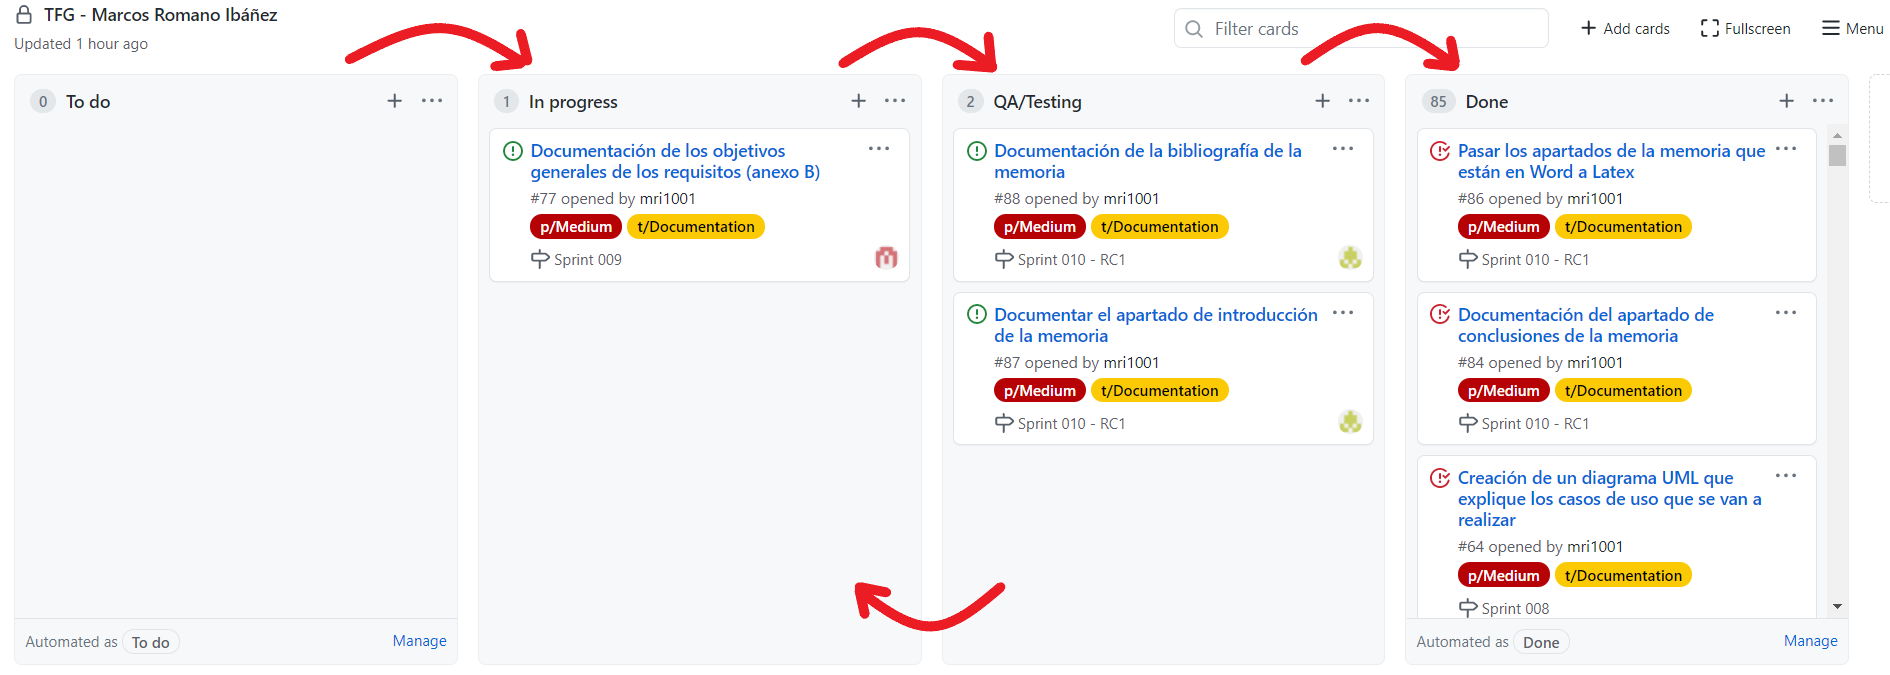
\includegraphics[scale=0.3]{Anexos/Anexo_A/Tablero_Kanban}
\caption{Captura de pantalla del tablero Kanban utilizado}
\end{figure}
\clearpage

\subsection{Fases del desarrollo}
Proyecto consta de tres fases separadas del desarrollo:
\begin{itemize}
\item
La fase de desarrollo del proyecto en la que se implementarán las mecánicas y los elementos del juego. Esta fase es la que más tiempo llevará, durando desde el 1 de febrero de 2021 hasta el 16 de mayo de 2021. Salvo por algunos bugs que quedaron pendientes de solucionar, los objetivos planteados para esta fase se cumplió satisfactoriamente.
\item
La fase de beta en la que se considera que el juego ya ha tomado forma como producto software y se entra a una fase centrada en la solución de bugs y documentación de la memoria. Esta fase duró desde el 17 de mayo de 2021 hasta el 6 de junio de 2021.\\
Durante esta fase se realizaron refactorizaciones (facilitan encontrar cambios), corrigieron bugs, se documentó la memoria y se añadieron recursos estéticos para mejorar la sensación de juego (principalmente sonidos).\\
Se invirtió demasiado tiempo en la implementación de los recursos que mejorasen la sensación de fuego (sobre todo la opción de modificación del volumen de la música) dedicándose poco tiempo a la memoria y ralentizando el cierre del proyecto.
\item
La fase de "Release candidate" que durará una semana donde comprobará que el desarrollo está listo, el código es accesible y el proyecto se puede descargar y ejecutar satisfactoriamente. Esta fase requerirá más trabajo del esperado ya que el retraso generado en la fase de beta ha obligado a arrastrar algunas de las tareas de esta a la "Release candidate". Sin embargo este retraso es más asumible debido a que se ha hecho la planificación temporal contando con un colchón de tiempo por si algún contratiempo retrasaba el proyecto.
\end{itemize}

\subsection{Cuellos de botellas}
Durante el desarrollo del proyecto se han encontrado tres cuellos de botellas en los que la realización de ciertas tareas ha llevado más tiempo del esperado:
\begin{itemize}
\item
La implementación del Player: La implementación del Player y todas las mecánicas relativas a este se tenía la percepción de que en 25-30 horas estarían implementadas. Sin embargo este proceso se alargó hasta las 48 horas.
\item
La implementación del sistema de colisiones estaba planeada para durar una semana de trabajo. Sin embargo se alargó hasta las dos.
\item
No estaba planeado añadir la opción de modificación del volumen de la música. Añadir esta tarea improvisada sobre la marcha, requirió de dos días que estaba planeado se dedicasen a tareas no improvisadas.
\end{itemize} 

\section{Estudio de viabilidad}
A continuación se va a proceder a realizar el estudio de viabilidad del proyecto. Dejar claro que este estudio de viabilidad no va a ser representativo de un estudio de viabilidad de un videojuego, ya que este TFG se ha centrado sobre todo en el punto de vista del programador obviando el resto de vertientes del proyecto como el apartado artístico o sonoro en los cuales se ha hecho uso de recursos de la comunidad gratuitos, de manera que los sueldos y otros gastos asociados a estos trabajadores no van a constar en el estudio de viabilidad económica.

Otro tema que diferirá de otros videojuegos desarrollados con Unity será que si en el último ejercicio fiscal los ingresos fueron superiores a 100.000 dolares americanos, se está obligado a comprar la edición profesional de Unity \cite{FAQUnity}. Al no comercializar el juego no es necesario estar pendiente de estos gastos. Presuponiendo también que es el primer producto desarrollado con Unity no habrá precedentes que obliguen a obtener la licencia profesional de Unity.

\subsection{Viabilidad económica}
Se va a valorar la viabilidad económica del proyecto desde el punto de vista económico. Para ello se evaluarán dos aspectos: los costes y los beneficios.\\
Los cálculos se harán asumiendo que el proyecto lo lleve a cabo una empresa y que se tenga liquidez suficiente como para no requerir financiamiento.

\subsubsection{Costes}
\textbf{Costes de recursos humanos:}
El salario medio de un programador de videojuegos en España es de 32.100 € \cite{Sueldo}. Sin embargo el sueldo varía mucho de un programador senior a uno junior. Se va a asumir que en este caso el programador es junior (es un alumno de 4º). El sueldo neto medio mensual de un programador junior es de 1.160 €.

\begin{figure}[h]
\centering
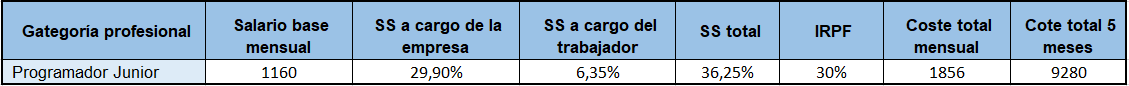
\includegraphics[scale=0.6]{Anexos/Anexo_A/Sueldo_trabajador}
\caption{Tabla de Excel con el sueldo calculado del trabajador}
\end{figure}

\textbf{Activos:}
El único activo que ha sido necesario para el desarrollo del proyecto ha sido el ordenador portátil en el que se ha creado el videojuego. Se estima que la vida útil de este activo será de 5 años, con lo que se amortizará en ese tiempo. En los 5 meses que ha durado el proyecto el coste de amortización del portátil es de 100 €

Las ventas no superarán los 100.000 €, así no hará falta pagar la versión profesional de Unity, resultando el software utilizado gratuito.

\begin{figure}[h]
\centering
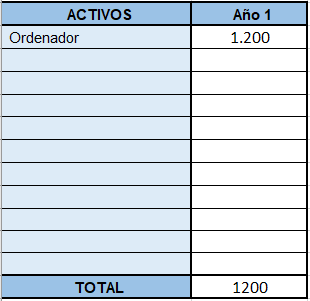
\includegraphics[scale=1]{Anexos/Anexo_A/Activos}
\caption{Tabla de Excel con los activos del proyecto}
\end{figure}

\subsubsection{Beneficios}
La media de unidades vendidas de por los videojuegos indies (desarrollados por muy pocas personas) está en torno a las 1.500 € unidades \cite{Unidades}. Si se desea vender el juego, el precio máximo que podría alcanzar es de 2€ por copia vendida, generando 3.000 € de ingresos.

\subsubsection{Balance}
El proyecto actualmente no es viable económicamente. Sin embargo cabe destacar que el principal motivo de esto es el precio del juego (2 euros). Es un precio bajo, pero actualmente tiene muy poco contenido el juego y no tiene sentido pedir más dinero por él.\\
Dejar claro también que con un 2 meses de producción (centrados en generar contenido jugable) más el juego se podría cobrar dignamente a 5 € y con otros 4 meses a 10 € o incluso 15 €.

\textbf{Balance actual:}
\begin{figure}[h]
\centering
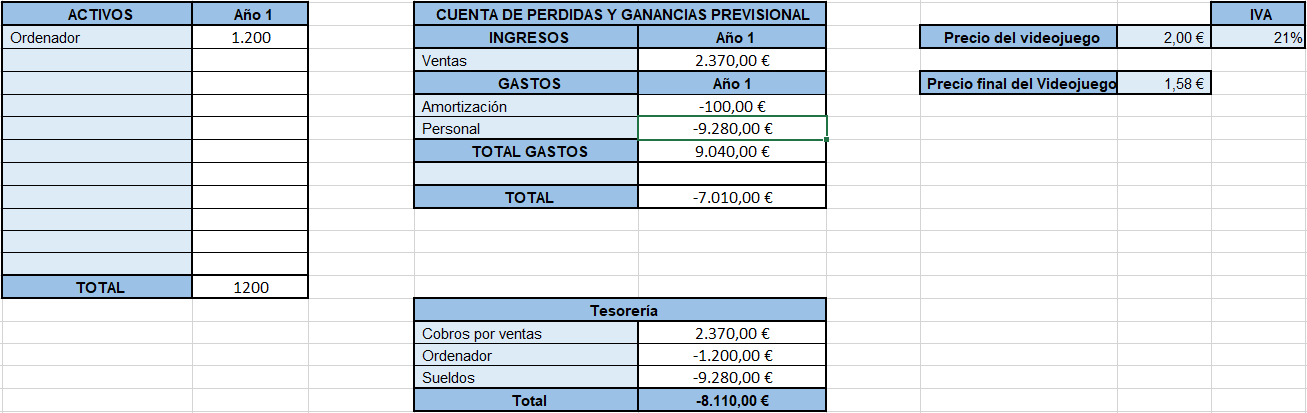
\includegraphics[scale=0.45]{Anexos/Anexo_A/Balance_actual}
\caption{Tabla de Excel con el balance del proyecto}
\end{figure}

\textbf{Balance a los 2 meses:}
\begin{figure}[h]
\centering
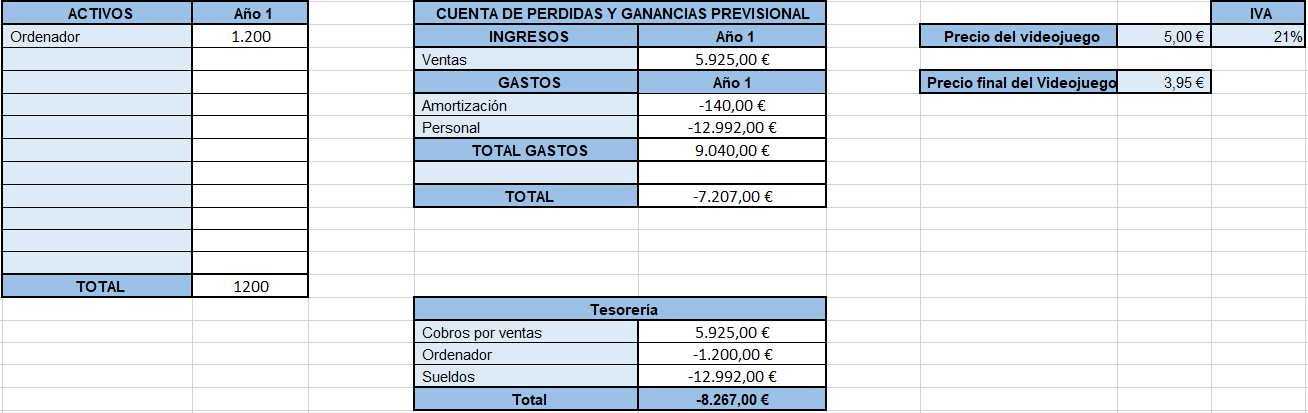
\includegraphics[scale=0.45]{Anexos/Anexo_A/Balance_2meses}
\caption{Tabla de Excel con el balance del proyecto con 2 meses más de desarrollo}
\end{figure}

\textbf{Balance a los 4 meses}
A los 4 meses de trabajo hay dos opciones:

Que el producto terminado posea el contenido suficiente pero su calidad deje algo que desear, en cuyo caso el juego se cobrará a 10 €.

\clearpage
\begin{figure}[h]
\centering
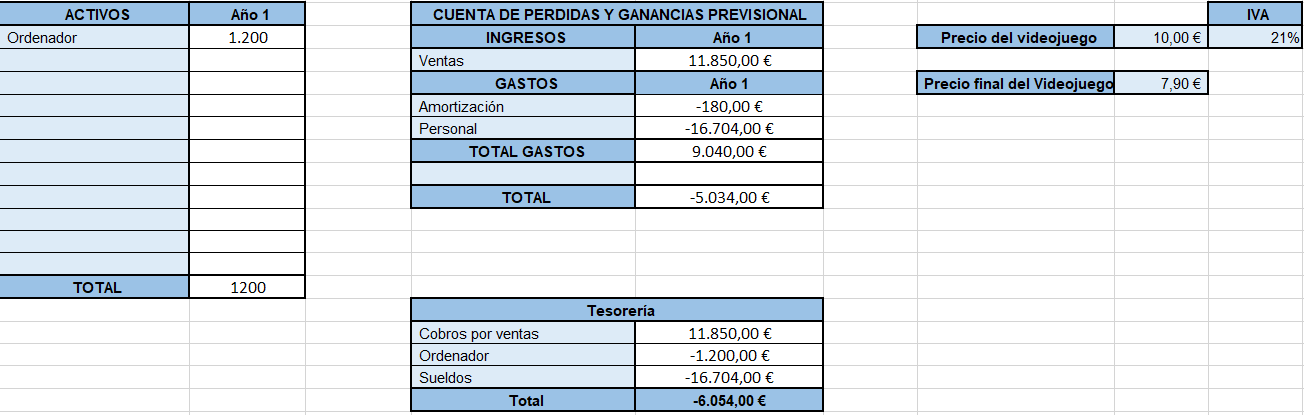
\includegraphics[scale=0.45]{Anexos/Anexo_A/Balance_4meses}
\caption{Tabla de Excel con el balance del proyecto con 4 meses más de desarrollo (precio del videojuego 10 €)}
\end{figure}

Que el producto terminado posea el contenido suficiente y haya sobrado tiempo para mejorar el apartado artístico. La calidad del juego es buena y se puede pedir 15 € por él.
\begin{figure}[h]
\centering
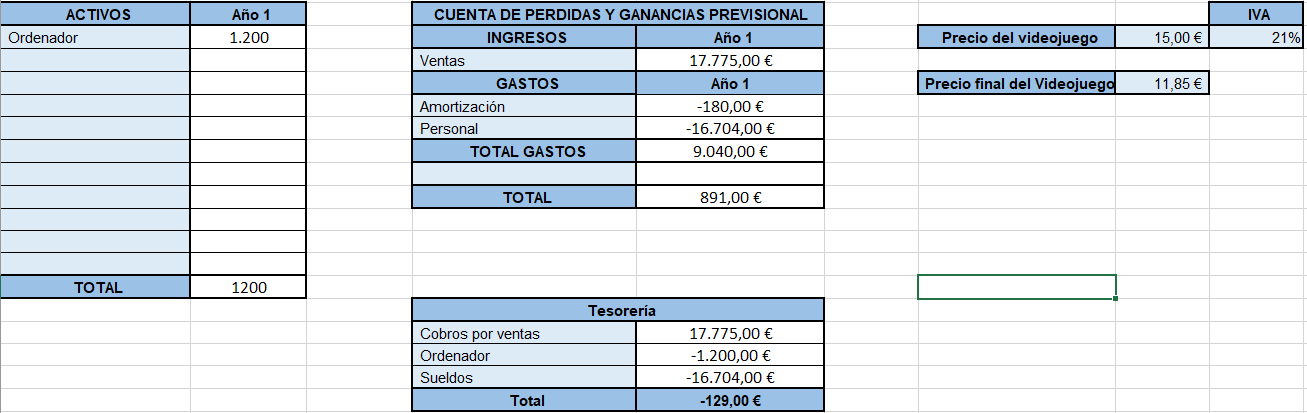
\includegraphics[scale=0.45]{Anexos/Anexo_A/Balance_4meses_optimista}
\caption{Tabla de Excel con el balance del proyecto con 4 meses más de desarrollo (precio del videojuego 15 €)}
\end{figure}

\subsection{Viabilidad legal}
En cuanto a la viabilidad legal, afortunadamente para este proyecto es sencillo el marco legal.

Los derechos de autoría corresponderán al desarrollador del videojuego y los de explotación a también a él. En caso de trabajar para una empresa los derechos de explotación se transmitirán a esta \cite{PropiedadIntelectual}.

Los elementos artísticos utilizados en el videojuego han sido obtenidos de personas que los han cedido para su libre uso. Todo este contenido se han regido por distintas leyes de CopyRigth, pero todas las estas leyes permiten su libre uso pero requiriendo mencionar al autor.

\clearpage
Esas leyes son:
\begin{itemize}
\item
Attribution 4.0 International (\url{https://creativecommons.org/licenses/by/4.0/})
\item
Attribution 3.0 Unported (\url{https://creativecommons.org/licenses/by/3.0/})
\item
Attribution 2.0 Generic (\url{https://creativecommons.org/licenses/by/2.0/})
\item
Attribution 1.0 Generic (\url{https://creativecommons.org/licenses/by/1.0/})
\end{itemize}
\apendice{Especificación de Requisitos}

\section{Introducción}

\section{Objetivos generales}

\section{Catalogo de requisitos}
\subsection{Requisitos funcionales}
Los requisitos funcionales especificarán cual es el funcionamiento que se espera del producto. Se concretarán a continuación.

\begin{itemize}
\item
\textbf{RF-1 Gestión de menús:}El jugador deber poder navegar por los menús.

\begin{itemize}
\item
\textbf{RF-1.1 Navegación entre pantallas:} Las pantallas deben de permitir navegar a otras pantallas (de manera directa o indirecta).
\end{itemize}

\item
\textbf{RF-2 Gestión del menú principal:} Deberá haber un menú principal que sea la primera escena que se muestre en el videojuego.

\begin{itemize}
\item
\textbf{RF-2.1 Selección de nivel:} Debe de poderse acceder a cualquier nivel desde el menú principal.
\end{itemize}

\begin{itemize}
\item
\textbf{RF-2.2 Cierre de la aplicación:} Se debe de poder cerrar la aplicación desde el menú principal.
\end{itemize}

\begin{itemize}
\item
\textbf{RF-2.3 Viaje al menú de opciones:} Se puede viajar desde el menú principal al menú de opciones.
\end{itemize}

\item
\textbf{RF-3 Gestión del menú de opciones:} Deberá haber un menú de opciones que permita modificar aspectos generales del juego. Desde el menú de opciones se debe poder volver al menú principal.

\item
\textbf{RF-4 Gestión de niveles:} Los niveles deben de contener todos los elementos necesarios y obligatorios de un nivel.

\begin{itemize}
\item
\textbf{RF-4.1 Controlar un avatar:} Debe de haber un avatar controlable por el jugador que realice las operaciones que le indique el jugador.
\end{itemize}

\begin{itemize}
\item
\textbf{RF-4.2 Zonas de muerte:} Debe haber zonas que maten al avatar del jugador cuando entre en contacto con ellas y devuelvan el nivel a un estado inicial.
\end{itemize}

\begin{itemize}
\item
\textbf{RF-4.3 Zonas de victoria (meta):} Debe haber zonas en las que, al entrar, se considere el nivel terminado y se vuelva al menú principal.
\end{itemize}

\begin{itemize}
\item
\textbf{RF-4.4 Gestión del menú de pausa:} Se debe poder acceder al menú de pausa, que parará la ejecución del nivel.

\begin{itemize}
\item
\textbf{RF-4.4.1 Abrir el menú de pausa:} Se deberá de poder abrir el menú de pausa, lo que pausara la ejecución del nivel.
\end{itemize}

\begin{itemize}
\item
\textbf{RF-4.4.2 Operaciones del menú de pausa:} Se deben de poder realizar las mismas operaciones que en el menú de opciones.
\end{itemize}

\begin{itemize}
\item
\textbf{RF-4.4.3 Cerrar el menú de pausa:} Se deberá poder cerrar el menú de pausa, lo que reanudará la ejecución del nivel.
\end{itemize}
\end{itemize}

\begin{itemize}
\item
\textbf{RF-4.5 Manipulación de la gravedad:} Debe de ser posible manipular la gravedad del nivel.
\end{itemize}

\begin{itemize}
\item
\textbf{RF-4.6 Manipulación del tiempo:} Debe de ser posible modificar la escala de tiempo que afecta al nivel.
\end{itemize}

\begin{itemize}
\item
\textbf{RF-4.7 Aplicación de impulsos:} Se debe poder aplicar impulsos que varíen la trayectoria que lleva un objeto.
\end{itemize}

\begin{itemize}
\item
\textbf{RF-4.8 Obstáculos:} Puede haber obstáculos que maten al avatar jugable cuando entre en contacto con ellos.
\end{itemize}

\begin{itemize}
\item
\textbf{RF-4.9 Portales:} Puede haber portales que teletransporten al avatar jugable desde el punto en el que se encuentra a otro que corresponderá con otro portal.
\end{itemize}
\end{itemize}

\begin{itemize}
\item
\textbf{RF-5 Gestión del avatar del jugador:} El jugador debe contar con un avatar controlable por el este. El avatar debe ser capaz de: saltar, moverse, realizar un acelerón y activar el tiempo bala.
\end{itemize}

\subsection{Requisitos no funcionales}
Al ser el producto a entregar un videojuego (un software de ocio), resulta clave especificar que requisitos no funcionales se van a tener en cuenta.

\begin{itemize}
\item
\textbf{Facilidad de uso:} Un videojuego cuyo uso no sea sencillo y cómodo puede perder muchos jugadores por esa única razón. Es clave que los jugadores tengan una experiencia agradable cuando interactúen con el juego.

\item
\textbf{Soporte:} Los cambios y actualizaciones del videojuego tienen que ser trasparentes al usuario, pues no tiene necesidad de conocer como funciona internamente el juego, sino solo abrir el ejecutable y disfrutar del juego.

\item
\textbf{Apariencia o interfaz externa (\textit{look and feel}):} No se ha especificado un diseño de interfaz, sin embargo en el mundo de los videojuegos hay un modelo general muy establecido. Es lógico adoptarlo para ofrecerle al jugador una experiencia que le resulte familiar.

\item
\textbf{Escalabilidad:} En un videojuego se van a ir añadiendo continuamente funcionalidades sobre el código para poder implementar todas las mecánicas, tanto definidas como que puedan surgir en el futuro. Por ello el código debe ser fácil de mantener y extender.
\end{itemize}


\section{Especificación de requisitos}



\apendice{Especificación de diseño}

\section{Introducción}
En este apartado se van a explicar elementos del diseño del proyecto que explican su funcionamiento y estructura.

\section{Trabajo propio vs trabajo ajeno}
Antes de nada es necesario mencionar que este trabajo ha partido de una platilla que ofrece Unity como punto de partida. Esa plantilla se llama Platformer Microgame y se puede añadir a tus assets en el siguiente enlace:\\
 \url{https://assetstore.unity.com/packages/templates/platformer-microgame-151055?_gl=1*cat3jy*_ga*NTAyOTIzMjY4LjE2MTIzNTE0Nzk.*_ga_1S78EFL1W5*MTYyMzE0MTIwMy41LjAuMTYyMzE0MTIwMy42MA..&_ga=2.202220375.778563316.1623141206-502923268.1612351479
}.\\ 
De esta plantilla se ha conservado sobre todo los elementos estéticos, pero también se ha conservado la clase Simulation y los eventos que esta lanza.

\subsection{Clase Simulation}
La calse Simulation es una clase encargada de manejar los eventos del juego. El objeto GameController hace uso de esta clase para ir ejecutando los eventos a medida que entran en cola. Esta clase tiene una particularidad de C\#. Simulaion es una “partial class”. Esto permite que la clase Simulation se construya en varios ficheros distintos. Para el funcionamiento de la clase Simulation, esta hace uso de otras dos subclases: Simulation.Event y Simulation.InstanceRegister. Se va a explicar a continuación porque son clases que se consideran importantes y claves para entender el funcionamiento de la arquitectura del videojuego.

\textbf{Simulation:} Este fichero contiene la estructura principal del funcionamiento de Simulation. Simulation es una clase estática con una cola, también estática, que guarda eventos (clase Event) y los libera cuando GameController llama al método tick(). Este fichero tiene el método tick() y los métodos necesarios para añadir y remover elementos de la cola. 

\textbf{Simulation.Event:} Contiene la clase interna Event que se encarga de ejecutar el comando asociado a ese evento. De esta clase de la que heredan todos los eventos que saltan durante la ejecución del juego (como por ejemplo EnemyDeath, el evento que salta cuando el jugador muere). Los eventos se guardan en su mayoría en la carpeta Assets/Scripts/Gameplay.

\textbf{Simulation.InstanceRegister:} Contiene la clase InstanceRegister. Esta clase simplemente devuelve una instancia nueva de un objeto cualquiera. Esta clase esta creada para que Simulation pueda crear singletons (patrón de diseño) de clases. Es utilizado para que todas las clases trabajen sobre el mismo modelo. Ese modelo es un script denominado PlataformerModel con una clase que exclusivamente tiene una serie de atributos (como el Player, las cámaras o el punto de aparición del jugador) que serán utilizados por varias clases.

\subsection{Eventos}
Los eventos son toda las clases que heredan de Simulation.Event. Todos los eventos se encuentran en la carpeta Assets/Scripts/Gameplay. Casi todas las clases evento del proyecto se han mantenido intactas de Platformer Microgame, sin embargo algunes eventos han sido modificados y otros añadidos.
Eventos modificados:
\begin{itemize}
\item
DisablePlayerInput.
\item
EnablePlayerInput.
\item
PlayerDeath.
\item
PlayerEnteredVictoryZone.
\end{itemize}
Eventos añadidos:
\begin{itemize}
\item
SetGameInitialState: Evento que se lanza para forzar volver la escena al estado inicial.
\item
PlayerObstacleCollision: Evento que salta cuando el Player colisiona con un obstáculo. Este evento mata al jugador.
\item
LoadGameMenu: Evento que carga la escena del menú principal y cambia a ella.
\end{itemize}

\section{Pseudocódigo}
Se va a mostrar a continuación el pseudocódigo de las mecánicas que se han implementado a modo de resumen que ilustre de forma simple la implementación de estas.

\subsection{Modificaciones gravitatorias}
\subsubsection{Obstáculo superdenso}

\subsubsection{Inversor de gravedad}

\begin{figure}[h]
\centering
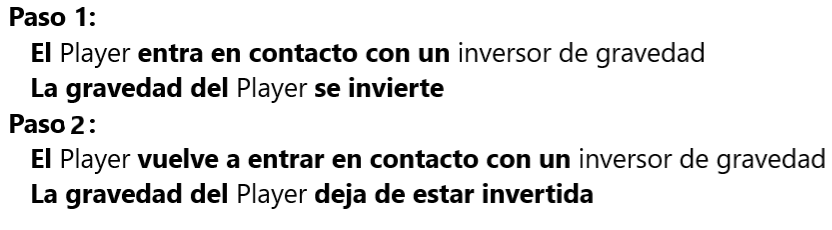
\includegraphics[scale=0.7]{Anexos/Anexo_C/Pseudocodigo_inversor}
\caption{Pseudocódigo que resume el funcionamiento del inversor de gravedad}
\end{figure}

\subsection{Movimiento de los obstáculos}
\subsubsection{Obstáculos estático}
Este obstáculo no se mueve.

\clearpage
\subsubsection{Obstáculos que siguen una rutina}

\begin{figure}[h]
\centering
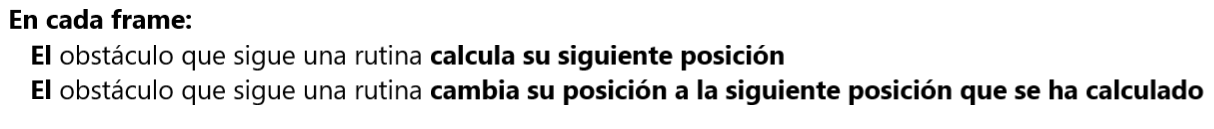
\includegraphics[scale=0.6]{Anexos/Anexo_C/Psudocodigo_rutina}
\caption{Pseudocódigo que resume el movimiento del obstáculo que sigue una rutina}
\end{figure}

\subsubsection{Obstáculos móviles}

\begin{figure}[h]
\centering

\includegraphics[scale=0.55]{Anexos/Anexo_C/Pseudocodigo_movil}
\caption{Pseudocódigo que resume el movimiento del obstáculo móvil}
\end{figure}

\subsection{Portales}
Para una de pareja de portales Portal1 y Portal2 enlazados entre sí.

\begin{figure}[h]
\centering
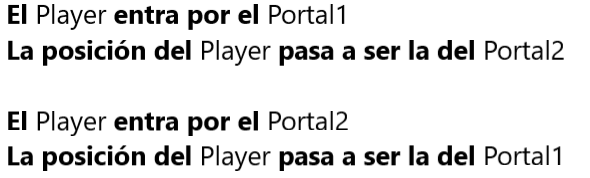
\includegraphics[scale=1]{Anexos/Anexo_C/Pseudocodigo_portal}
\caption{Pseudocódigo que resume el funcionamiento de los portales}
\end{figure}
\clearpage

\subsection{Creadores de impulso}
\subsubsection{Partícula de impulso}

\begin{figure}[h]
\centering
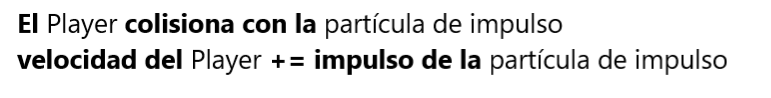
\includegraphics[scale=1]{Anexos/Anexo_C/Pseudocodigo_particula}
\caption{Pseudocódigo que resume el funcionamiento de la partícula de impulso}
\end{figure}

\subsubsection{Plataforma de salto}

\begin{figure}[h]
\centering

\includegraphics[scale=0.7]{Anexos/Anexo_C/Pseudocodigo_plataforma}
\caption{Pseudocódigo que resume el funcionamiento de la plataforma de salto}
\end{figure}

\subsubsection{Amplificador de impulso}

\begin{figure}[h]
\centering

\includegraphics[scale=0.7]{Anexos/Anexo_C/Psudocodigo_ampificador}
\caption{Pseudocódigo que resume el funcionamiento del amplificador de impulso}
\end{figure}

\clearpage
\subsection{Animación de Sprites}
\subsubsection{SpriteAnimator}

\begin{figure}[h]
\centering

\includegraphics[scale=1]{Anexos/Anexo_C/Psudocodigo_loop_anim}
\caption{Pseudocódigo que resume el funcionamiento del animador en loop}
\end{figure}

\subsubsection{OneTimeAnimator}

\begin{figure}[h]
\centering

\includegraphics[scale=1]{Anexos/Anexo_C/Psuedocodigo_animador}
\caption{Pseudocódigo que resume el funcionamiento del animador de un solo uso}
\end{figure}

\subsection{Modificadores temporales}
\subsubsection{Tiempo bala}

\begin{figure}[h]
\centering
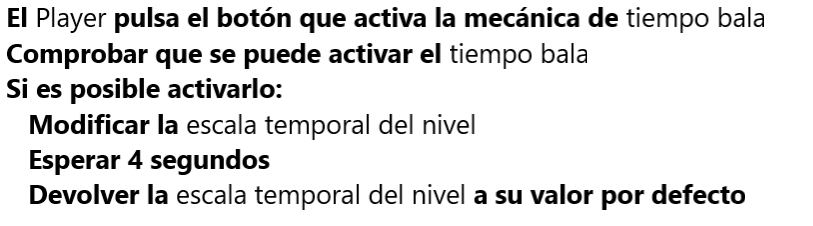
\includegraphics[scale=0.6]{Anexos/Anexo_C/Pseudocodigo_tiempo_bala}
\caption{Pseudocódigo que resume el funcionamiento de la mecánica de tiempo bala}
\end{figure}

\clearpage
\subsubsection{Zonas de gravitación temporal}

\begin{figure}[h]
\centering
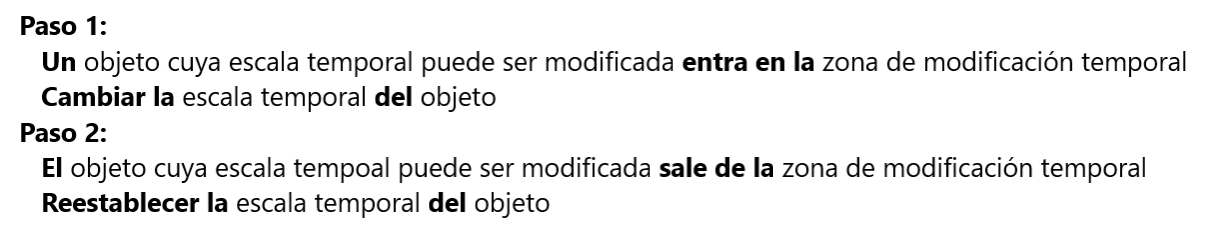
\includegraphics[scale=0.6]{Anexos/Anexo_C/Pseudocodigo_zona}
\caption{Pseudocódigo que resume el funcionamiento de las zonas de gravitación temporal}
\end{figure}

\section{Diseño de datos}
Los datos necesarios para el desarrollo de un videojuego son los Sprites y los audios utilizados durante su ejecución.

Para utilizar estos recursos en Unity se hace uso de los AudioSources \cite{AudioSource} y los SpriteRenderers \cite{SpriteRenderer}.

\subsection{AudioSource}
La clase AudioSource es la case de la que hace uso Unity para reproducir audios. Esta clase tiene un atributo público AudioClip que contendrá el audio que se va a reproducir. Se puede saber si el audio se esta reproduciendo con el atributo booleano isPlaying.\\
Se puede modificar el volumen de reproducción de todo audio reproducido con ese AudioSource.

Los métodos de reproducción de audios son los siguientes:
\begin{itemize}
\item
Play: reproduce el audio asociado al AudioSource (AudioSource.AudioClip).
\item
PlayDelayed: reproduce el audio asociado al AudioSource despues del tiempo pasado por parámetros.
\item
PlayOneShot: permite reproducir cualquier audio pasado como parámetro. El audio que se desea reproducir deberá estar encapsulado en una instancia de la clase AudioClip \cite{AudioClip} .
\end{itemize}

En el proyecto desarrollado AudioSource se ha usado para controlar el volumen del juego. Se ha creado una clase VolumeManager encargada de guardar y modificar el volumen general del juego y el volumen de la música.\\
Sin embargo, los AudioSources del juego están protegidos por clases envoltorio encargadas de modificar el volumen del juego de acuerdo a las opciones de juego.

\begin{figure}[h]
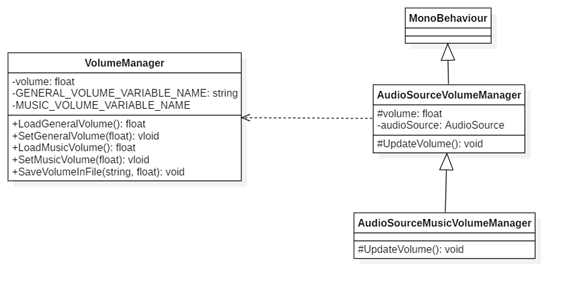
\includegraphics[scale=1]{Memoria/Aspectos_relevantes/Volumen_persistente/VolumeManager_UML}
\caption{Diagrama UML de las clases que hacen uso del AudioSource}
\end{figure}

\subsection{SpriteRenderer}
La clase SpriteRenderer es la encargada de hacer que se muestre una imagen en una zona del videojuego. Para poder mostrar las imágenes en Unity hay que utilizar la clase envoltorio Sprite. SpriteRenderer tiene un atributo público Sprite que contiene la imagen que mostrará ese SpriteRenderer.

En el proyecto se ha hecho uso de esta clase para mostrar imágenes estáticas y para mostrar animaciones.\\
Para crear las animaciones se ha creado dos clases SpriteAnimator y OneTimeAnimator. Estas clases simulan la animación intercalando a grandes velocidades un conjunto de imágenes. La diferencia entre estas dos clases es que SpriteAnimator reproduce una animación indefinidamente en bucle y OneTimeAnimator reproduce la animación una sola vez.

\begin{figure}[h]
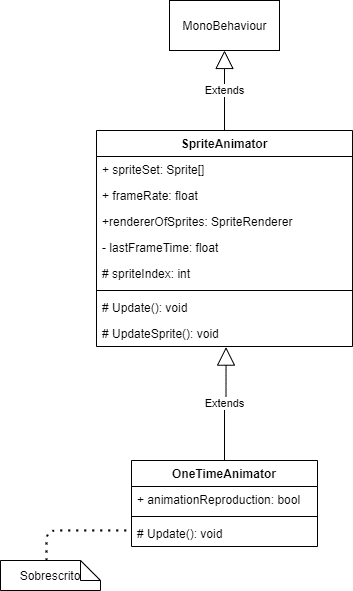
\includegraphics[scale=0.8]{Memoria/Aspectos_relevantes/Animadores/Herencia_animators}
\caption{Diagrama UML de las clases SpriteAnimator y OneTimeAnimator}
\end{figure}

\section{Diseño procedimental}
En este apartado se explicarán los algoritmos que se han desarrollado para el correcto funcionamiento del videojuego.

\subsection{Sistema de colisiones}
Para simular el sistema de colisiones se optó por utilizar la velocidad como elemento principal.

\clearpage
\begin{figure}[h]
\centering
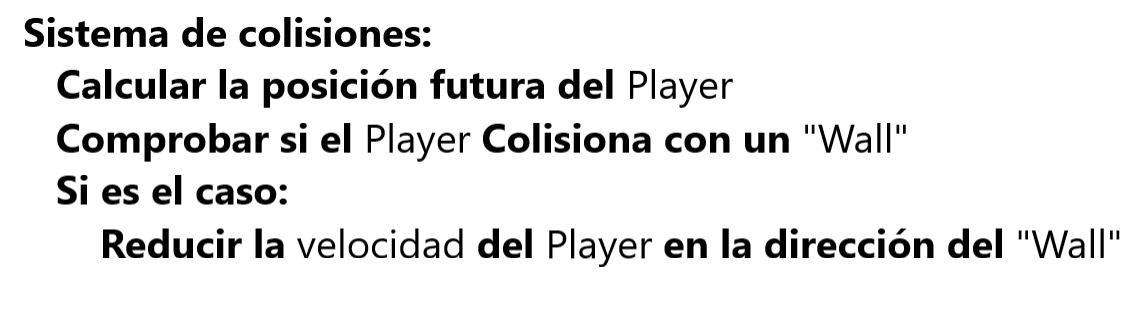
\includegraphics[scale=0.7]{Anexos/Anexo_C/Pseudocodigo_colisiones}
\caption{Pseudocódigo que resume el sistema de colisiones}
\end{figure}

Para saber si un KinematicObject va a colisionar con el suelo o un muro (se identifican los objetos con los que se desea chocar porque tienen asignada la layer “Wall”) se coge la velocidad del KinematicObject (se obtiene del atributo velocity del Rigidbody2D), que está representada en unidades/segundo. Con la velocidad que lleva el KinematicObject y su posición se puede deducir la siguiente posición en la que se encontrará.

Hay un método que se llama Physics2D.BoxCast con el que puedes crear un rectángulo en una región del espacio y comprobar si se colisiona con algún objeto. En caso de colisionar con un objeto se devuelve un objeto de la clase RayCastHit2D con toda la información relativa a la colisión. Hay un método similar a Physics2D.BoxCast que es Physics2D.BoxCastAll que hace lo mismo pero devolviendo un vector de RayCastHit2D con un elemento por cada objeto con el que has colisionado.

Se puede filtrar las colisiones por Layer, pudiendo solo tener en cuenta las colisiones con objetos que tengan asociada una Layer con el mismo nombre que el pasado por parámetro en el método. Para el sistema de colisiones solo se han tenido en cuenta los objetos con Layer igual a “Wall”.

Con el método Physics2D.BoxCastAll se va a crear un rectángulo del tamaño del Collider2D del KinematicObject en la siguiente posición en la que se encontrará el objeto y comprobarán cuántos objetos con Layer igual a “Wall” colisionarán en esa posición con el KinematicObject.

\clearpage
\begin{figure}[h]
\centering
\includegraphics[scale=1]{Memoria/Aspectos_relevantes/Sistema_Colisiones/Detección_colisiones}
\caption{Simulación del proceso de detección de colisiones}
\end{figure}

Una vez detectados con que muros se han colisionado (objetos con Layer igual a “Wall”) se va a simular el choque modificando la velocidad del KinematicObject poniendo a cero la velocidad en la dirección de la colisión del muro. Un ejemplo de aplicación sería un KinematicObject yendo a una velocidad marcada por el vector (1, -2), es decir 1 unidad hacia la derecha (eje x) y dos unidades hacia abajo (eje y). Si se detecta que se va a colisionar contra el suelo (un muro que está a los pies del KinematicObject) la velocidad debería establecerse al vector (1,0), es decir continuar el desplazamiento a la derecha pero cesar el movimiento hacia abajo.

Para calcular en qué dirección hay que limitar la velocidad se utiliza el vector normal de la recta creada por la pared más cercana del muro. Ese vector normal lo ofrece el objeto RayCastHit2D en su atributo “normal”.
Se va a añadir una figura explicativa:

\clearpage
\begin{figure}[h]
\centering
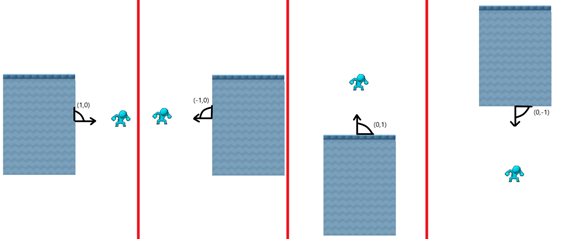
\includegraphics[scale=1]{Memoria/Aspectos_relevantes/Sistema_Colisiones/Vector_normal}
\caption{Vector normal del muro en función de la posición del KinematicObject}
\end{figure}

De la colisión del KinematicObject se encarga el objeto KinematicObjectCollisionManager, que tiene una referencia a KinematicObject y se encarga de llamar al método Physics2D.BoxCastAll y limitar la velocidad del KinematicObject en caso de colisión.

\begin{figure}[h]
\centering
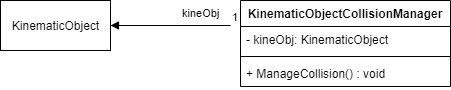
\includegraphics[scale=1]{Memoria/Aspectos_relevantes/Sistema_Colisiones/KinematicObjectCollisionManager_UML}
\caption{Diagrama UML del sistema de colisiones}
\end{figure}

\subsection{Modificaciones gravitatorias}
Durante la ejecución del juego puede ser que los objetos kinemáticos sufran modificaciones que varíen las fuerzas gravitatorias que los afectan. Estas modificaciones las provocan los modificadores de gravedad y no afectan a todos los elementos del juego sino a un objeto kinemático en concreto.

Dada esta premisa, se ha creado una clase KinematicObjectGravityManager encargada de la gestión de las modificaciones de gravedad que afectan al KinematicObject.

\begin{figure}[h]
\centering
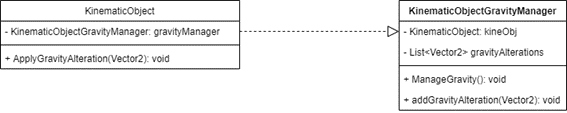
\includegraphics[scale=1]{Memoria/Aspectos_relevantes/Modificaciones_gravitatorias/KinematicObjectGravityManager_UML}
\caption{Diagrama UML de la clase encargada de la gestión de la gravedad del KinematicObject}
\end{figure}

KinematicObjectGravityManager va a funcionar mediante una lista a la que se van a ir añadiendo objetos de clase Vector2 que representarán las alteraciones de la gravedad. En cada llamada al método FixedUpdate de KinemticObject se recorre la toda la lista acumulando las alteraciones gravitatorias y se aplican esas alteraciones al efecto gravitatorio por defecto (Physics2D.gravity) y se simula la gravedad. Después de este proceso se vacía la lista.

\begin{figure}[h]
\centering
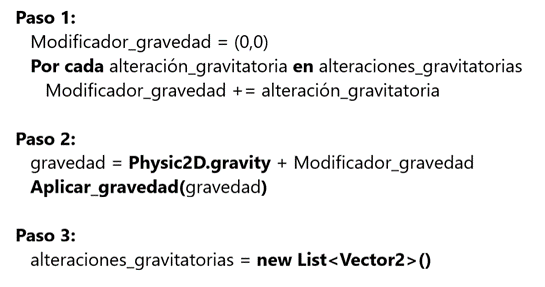
\includegraphics[scale=1]{Memoria/Aspectos_relevantes/Modificaciones_gravitatorias/Pseudocodigo_modificadores_gravedad}
\caption{Pseudocódigo del proceso de modificación de la gravedad del KinematicObject}
\end{figure}

Hay dos tipos de modificadores de gravedad: los obstáculos superdensos y los inversores de gravedad. La diferencia fundamental entre estos modificadores de gravedad es que los obstáculos superdensos aplican una modificación temporal mientras que los inversores de gravedad modifican la gravedad de forma permanente (o hasta que se cancele el efecto).

\subsection{TimeAffectedObjects}
Hay una serie de objetos que se ven afectados por las modificaciones temporales particulares. Estos objetos heredarán de la clase TimeAffectedObject. 

\begin{figure}[h]
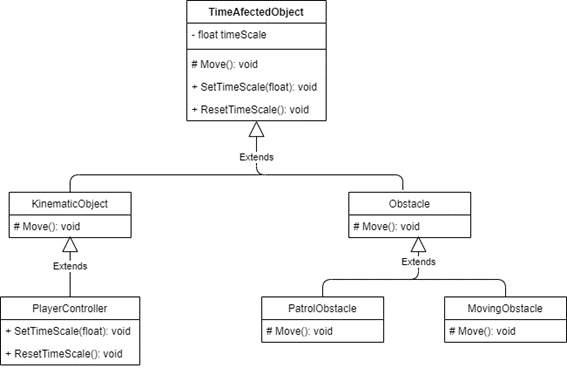
\includegraphics[scale=1]{Memoria/Aspectos_relevantes/Tiempo_bala/Herencia_TimeAffectedObject}
\caption{Clases que heredan de TimeAffectedObject}
\end{figure}

El movimiento de las clases que hereden de esta deberá implementarse en el método Move, pues será en ese método en el que se aplicará la modificación temporal al movimiento acelerándolo o ralentizándolo según toque.

Cuando el juego vuelva al estado inicial será necesario restablecer la escala temporal de todos los TimeAfectedObjects a la escala por defecto.

\begin{figure}[h]
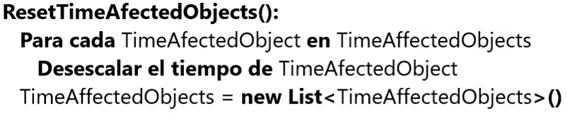
\includegraphics[scale=1]{Memoria/Aspectos_relevantes/Tiempo_bala/Pseudocodigo_TimeAffectedObject}
\caption{Pseudocódigo del método llamado para resetear los TimeAfectedObject}
\end{figure} 

\section{Diseño arquitectónico}
\subsection{GameController}
Se ha desarrollado una arquitectura específica para asegurar que los niveles jugables tienen están siempre en un estado estable de juego, y un proceso a seguir cada vez que se reinicia el nivel a su estado inicial.\\
Con este propósito se ha creado la clase GameController. Esta clase contiene dos elementos distintos al servicio del mismo propósito.

\begin{figure}[h]
\centering
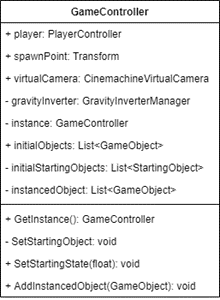
\includegraphics[scale=1]{Memoria/Aspectos_relevantes/GameController/GameController}
\caption{Diagrama UML de la clase GameController}
\end{figure}

\subsection{Variables de PlatformerModel}
La clase GameController contendrá una serie de atributos que, al iniciar la escena copiará en la clase PlatformerModel esos atributos. Estas variables son variables relevantes del nivel. Son movidas a la clase PlatformerModel para que todos los objetos de la escena puedan acceder a estas variables facilmente sin generar cadenas de mensajes para tener acceso a ellas.

Las variables de GameController que serán copiadas a PlatformerModel serán:
\begin{itemize}
\item
La CinemachineVirtualCamera que utiliza la escena (PlatformerModel.virtualCamera).
\item
El PlayerController asignado al avatar jugable (PlatformerModel.player).
\item
El objeto de tipo Transform asociado al punto de reaparición e inicio de escena del Player (PlatformerModel.spawnPoint).
\item
El GameController de la escena (PlatformerModel.gameController).
\item
El GravityInverterManager asociado a la escena \\ (PlatformerModel.gravityInverterManager).
\end{itemize}

\subsection{Estado inicial de juego}
Cuando el Player muera será necesario devolver el nivel al estado inicial en el que se encontraba al acceder a esa escena.\\
Para volver a este estado inicial será necesario:
\begin{itemize}
\item
Eliminar los objetos creados que no estaban instanciados al inicio del nivel.
\item
Devolver los objetos cuyo estado haya variado durante la ejecución del nivel a su estado inicial (un ejemplo sería devolver un obstáculo que sigue una rutina del punto en el que se encuentra al punto en el que empieza el juego).
\item
Instanciar objetos que estaban al inicio del nivel pero que ya no están instanciados.
\item
Devolver el Player a su posición inicial.
\end{itemize}

En la implementación del programa, se han tratado todos los objetos que debían ser devueltos a su estado inicial (salvo al Player) como el mismo tipo de objetos. Han sido guardados en una clase envoltorio que guarda el estado inicial del objeto. Estos objetos no serán los que estén en la escena, sino que en el estado inicial del juego se generarán clones de él en la escena.\\
Todos los objetos instanciados serán guardados en la lista instancedObjects para poder destruirlos cuando haya que reiniciar el nivel. Los objetos que se instancien durante la escena también serán añadidos a isntancedObjects.

\clearpage
\begin{figure}[h]
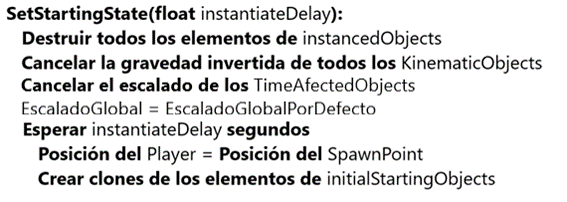
\includegraphics[scale=1]{Memoria/Aspectos_relevantes/GameController/Pseudocodigo_starting_objects}
\caption{Pseudocódigo de las operaciones realizadas al establecer el estado inicial del nivel}
\end{figure}

\subsection{Estados del Player}
El Player se comportará de distinta forma en función de en que situación se encuentre. Para facilitar la lógica del Player y el cambio en tiempo de ejecución del comportamiento de este, se ha aplicado el patrón de diseño Estado.

\begin{figure}[h]
\centering
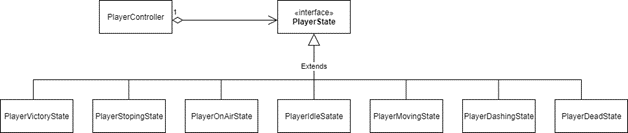
\includegraphics[scale=0.85]{Memoria/Aspectos_relevantes/Arquitectura_Player/Estados_Player}
\caption{Diagrama UML de la aplicación del patrón de diseño Estado en el Player}
\end{figure}

El Player puede estar en los siguientes estados:
\begin{itemize}
\item
PlayerIdleState: El Player está detenido sobre una superficie.
\item
PlayerOnAirState: El Player está en el aire.
\item
PlayerMovingState: El Player se está moviendo sobre una superficie.
\item
PlayerStopingState: El Player ha cesado el movimiento y se está deteniendo.
\item
PlayerDashingState: El Player está realizando el acelerón.
\item
PlayerVictoryState: El Player ha llegado a la meta.
\item
PlayerDeadState: El Player está muerto.
\end{itemize}

\begin{figure}[h]
\centering
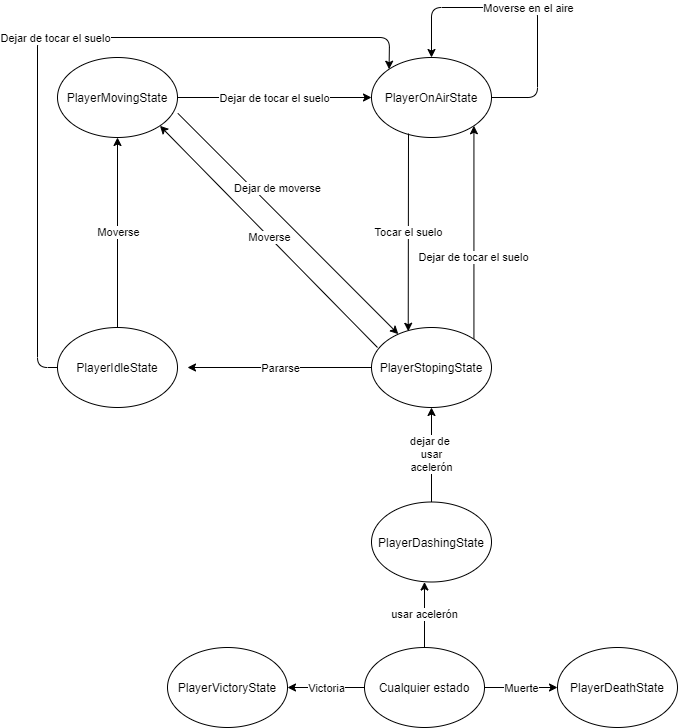
\includegraphics[scale=0.55]{Memoria/Aspectos_relevantes/Arquitectura_Player/Diagrama_de_estados}
\caption{Diagrama de transición entre estados del Player}
\end{figure}
\apendice{Documentación técnica de programación}

\section{Introducción}
Hay una serie de elementos relativos al proyecto que no tiene que ver estrictamente con el desarrollo, pero que pueden ser útiles conocer (tales como la estructura de ficheros, la importación y exportación del proyecto o la pruebas de sistema). Se explicarán a continuación. 

\section{Estructura de directorios}
Se va a comentar la estructura de ficheros del repositorio de GitHub que contiene todos los materiales relativos al proyecto.

\begin{itemize}
\item
/: Directorio raíz del repositorio.
\item
/docs: Directorio que contiene todos los ficheros relativos a la documentación.
\item
/docs/Latex: Carpeta con todos los ficheros necesarios para la generación de la memoria y los anexos con Latex.
\item
/docs/Latex/img: Contiene todas las imágenes que aparecerán el los ficheros generado en Latex.
\item
/docs/Latex/tex: Contiene los ficheros de Latex secundarios que utilizarán los principales para generar la memoria y los anexos.
\item
/game: Contiene la solución de Visual Studio con el código relativo al vidojuego desarrollado.
\item
/game/Assets: Contiene todos los ficheros de código en C\# y en formatos especializados de Unity necesarios para que Unity pueda exportar el juego correctamente.
\item
/game/Assets/Audio: Ficheros de audio del proyecto.
\item
/game/Assets/Character: Elementos estéticos exclusivos del Player.
\item
/game/Assets/Character/Animations: Animaciones que provee Platformer Microgame utilizadas en el Player.
\item
/game/Assets/Character/Sprites: Sprites del Player.
\item
/game/Assets/Environment: Sprites utilizados para crear los mapas de los niveles jugables.
\item
/game/Assets/ModAssets: Elementos estéticos extra que provee Platformer Microgame para ofrecer más variedad estética.
\item
/game/Assets/Prefabs: Contiene todos los prefabs del proyecto.
\item
/game/Assets/Scenes: Contiene todas las escenas que conforman el proyecto.
\item
/game/Assets/Scripts: Ficheros de C\# utilizados en el proyecto.
\item
/game/Assets/Scripts/Animation: Ficheros de C\# utilizados en el proyecto relativos a la animación de sprites.
\item
/game/Assets/Scripts/Core: Ficheros de C\# utilizados en el proyecto. Contiene las clases encargadas del funcionamiento básico de los niveles.
\item
/game/Assets/Scripts/Gameplay: Ficheros de C\# utilizados en el proyecto. Contiene las clases que son eventos de Simulation.
\item
/game/Assets/Scripts/GizmosUI: Ficheros de C\# utilizados en el proyecto. Contiene las clases utilizadas para mostrar los Gizmos en el editor.
\item
/game/Assets/Scripts/Mechanics: Ficheros de C\# utilizados en el proyecto. Contiene las clases que implementa las mecánicas del juego.
\item
/game/Assets/Scripts/Model: Ficheros de C\# utilizados en el proyecto. Contiene una clase con las variables que se consultarán durante los niveles.
\item
/game/Assets/Scripts/Sound: Ficheros de C\# utilizados en el proyecto. Contiene las clases encargadas de gestionar el audio.
\item
/game/Assets/Scripts/UI: Ficheros de C\# utilizados en el proyecto. Contiene todas las clases relativas a la interfaz de usuario.
\item
/game/Assets/Scripts/View: Ficheros de C\# utilizados en el proyecto. Contiene clases que ofrecen comportamientos que afectan de forma especial a como debería verse un objeto.
\item
/game/Assets/Sprites: Sprites del proyecto que no pertenecen a Platformer Microgame.
\item
/game/Assets/Scripts: Elementos usados para generar mapas mediante la herramienta Tilemap de Unity.
\end{itemize}

\section{Manual del programador}
\subsection{Ventanas de Unity}
Se van a listar a continuación una serie de ventanas del editor de Unity y se explicará su propósito.

\subsubsection{Console}
Consola interna de Unity que mostrará los print realizados por las clases Monobehaviour y errores y warnings de compilación y ejecución.

\clearpage
\begin{figure}[h]
\centering
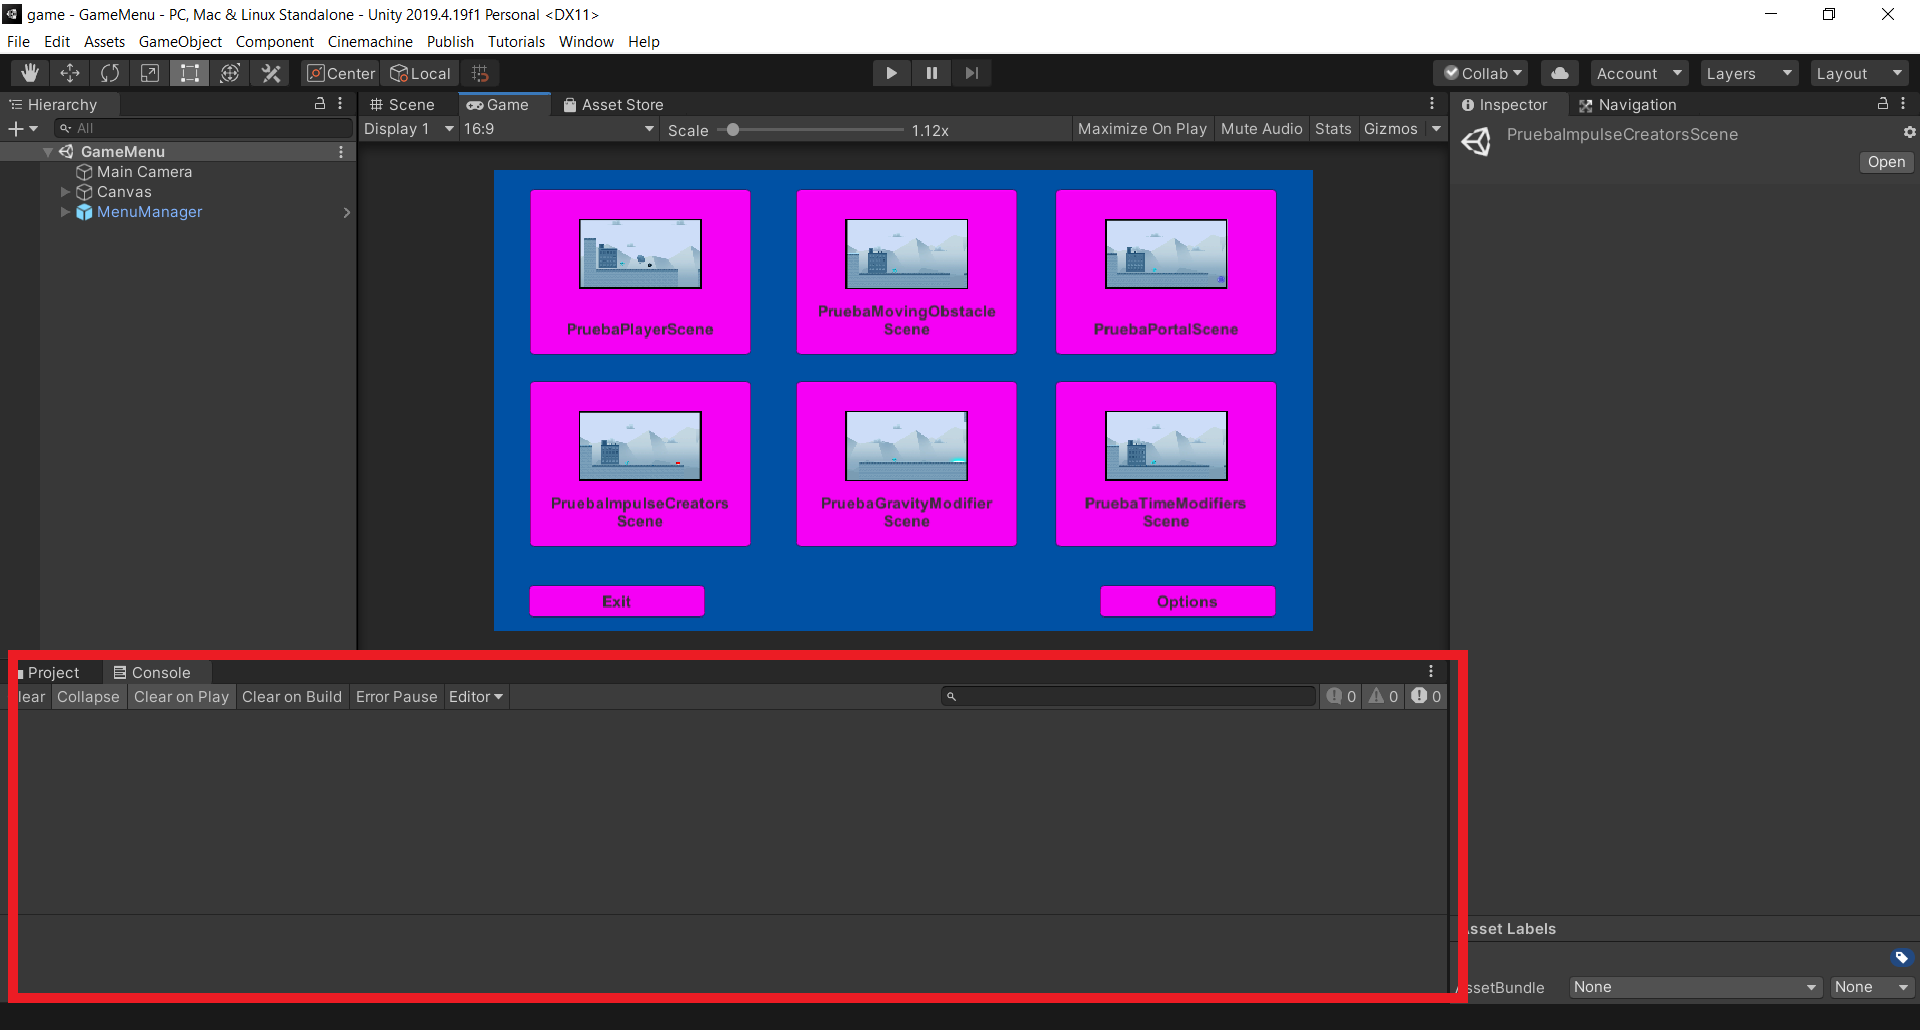
\includegraphics[scale=0.3]{Anexos/Anexo_D/Consola_Unity}
\caption{Consola de Unity}
\end{figure}

\subsubsection{Project}
Ventana que muestra todo el sistema de ficheros del proyecto que se está desarrollando.

\begin{figure}[h]
\centering
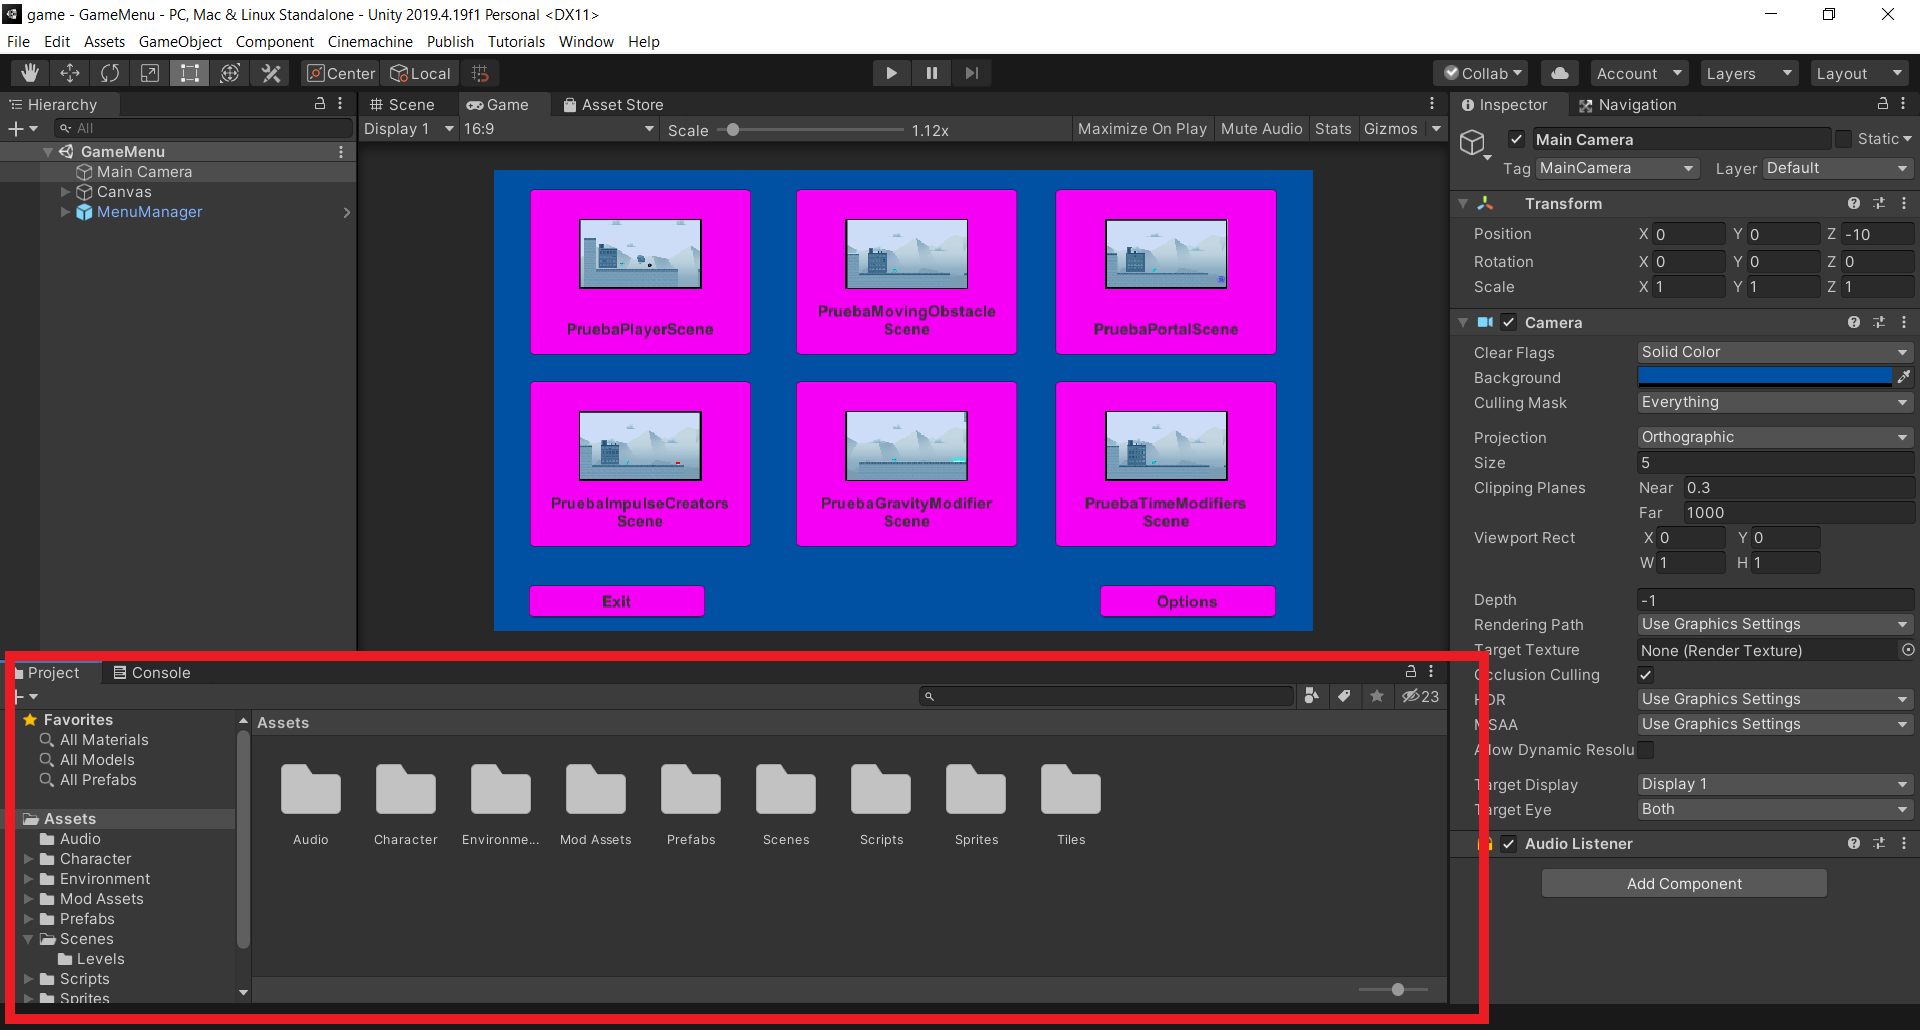
\includegraphics[scale=0.2]{Anexos/Anexo_D/Project}
\caption{Vetana ''Project'' de Unity}
\end{figure}
\clearpage

\subsubsection{Hierarchy}
Ventana que muestra los elementos que componen la escena y las dependencias padre-hijo entre estos.

\begin{figure}[h]
\centering
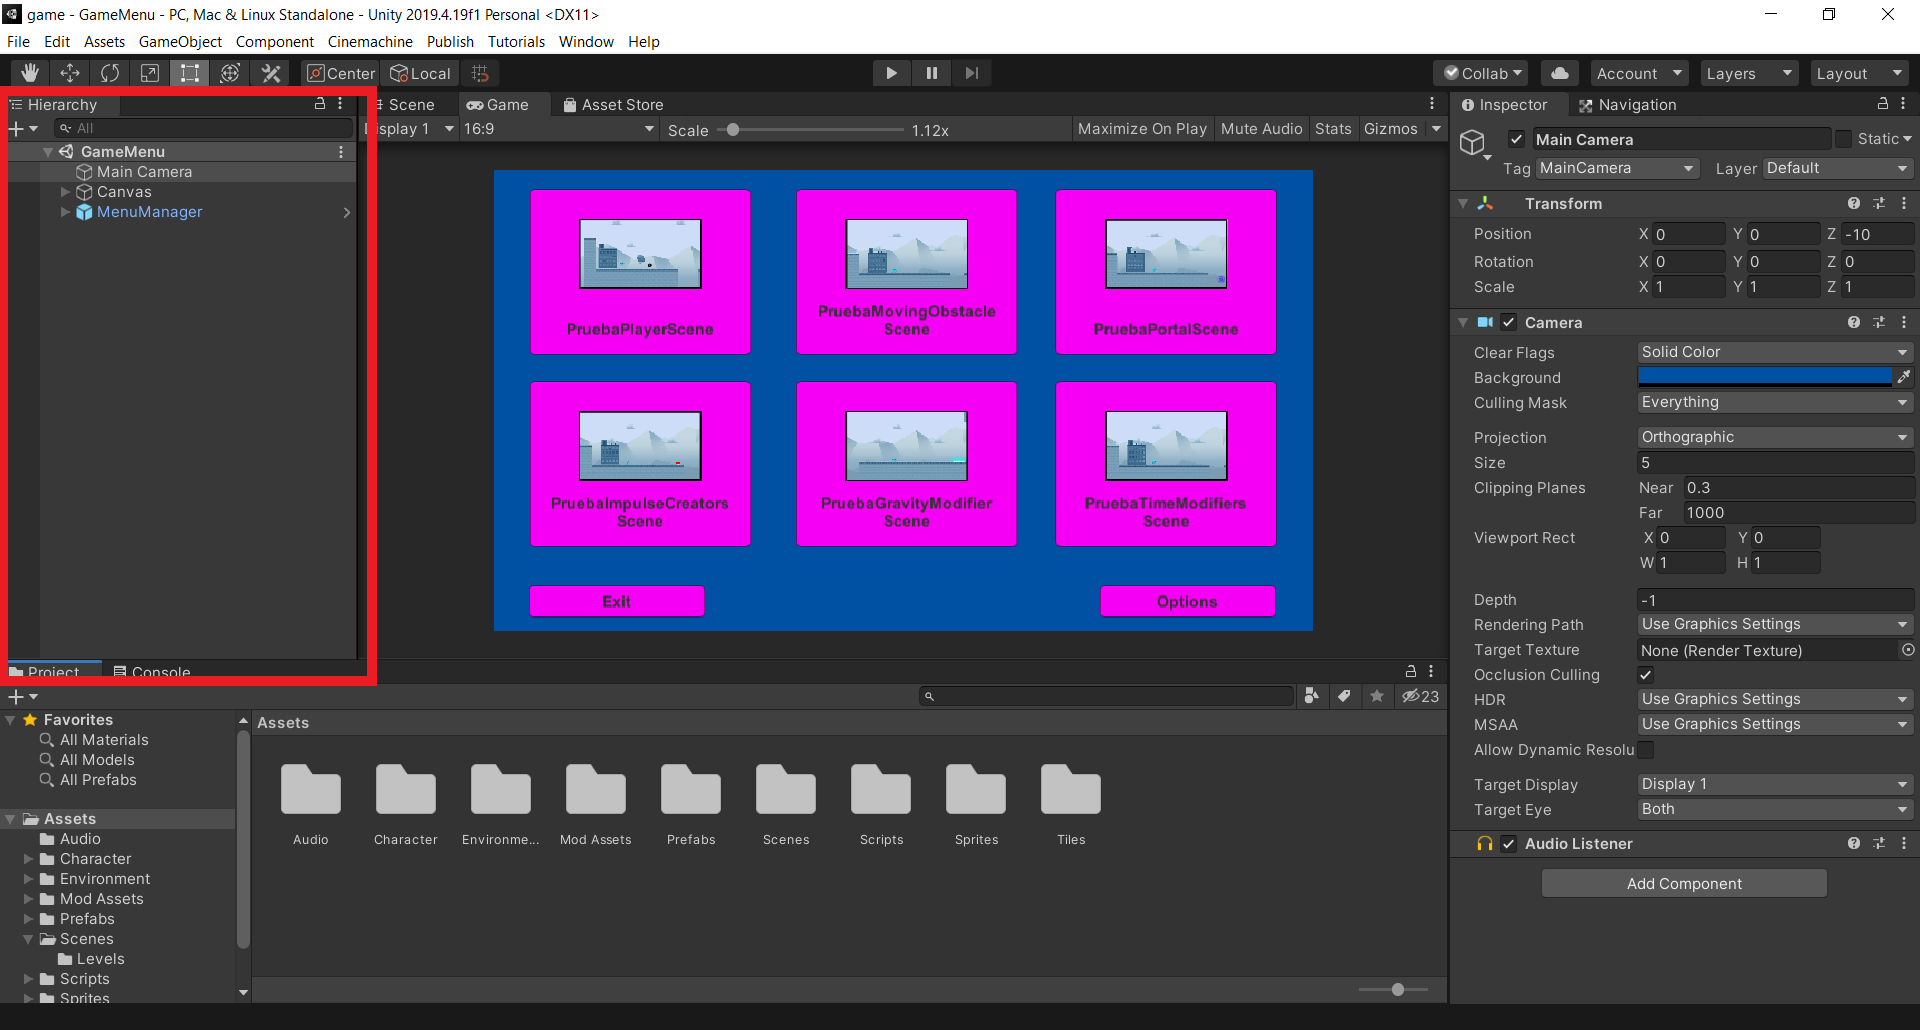
\includegraphics[scale=0.3]{Anexos/Anexo_D/Hierarchy}
\caption{Ventana ''Hierarchy'' de Unity}
\end{figure}

Estos elementos serán distintos para cada escena. Sin embargo en los niveles jugables tendrán una serie de elementos comunes:
\begin{itemize}
\item
MainCamera: Cámara encargada de mostrar por pantalla lo que el jugador debe ver.
\item
OptionsMenuCanvas: Estructura de objetos que conformarán el menú de pausa.
\item
GameController: Objeto encargado de que el juego mantenga un estado estable. Tiene un objeto hijo que es un reproductor de música.
\item
SpawnPoint: Punto de aparición del Player. También reaparecerá en este punto tras morir.
\item
Player: Avatar que controlará el jugador.
\item
CineachineConfiner: La cámara no se podrá desplazar más allá de los límites marcados por este objeto.
\item
CM vcam1: Objeto encargado del control del movimiento de la cámara.
\item
Grid: Contiene los Tilemaps que construyen el nivel. Tiene 4 objetos hijos: FarBackgroundTilemap para elementos muy alejados del nivel (montañas), BackgroundTilemap para elementos alejados del nivel (nubes), LevelTilemap para elementos que forman parte del nivel y se espera poder interactuar con ellos (suelos y paredes) y ElementsTilemap para elementos que forman parte del nivel, pero son puramente estéticos (árboles y edificios).
\item
Zones: zonas relevantes del nivel. Podrán ser de tres tipos: muros o suelos, zonas de muerte y zonas de victoria.
\end{itemize}

\subsubsection{Inspector del Objeto}
Ventana que muestra la información y ajustes de los componentes que conforman un GameObject seleccionado.

\begin{figure}[h]
\centering
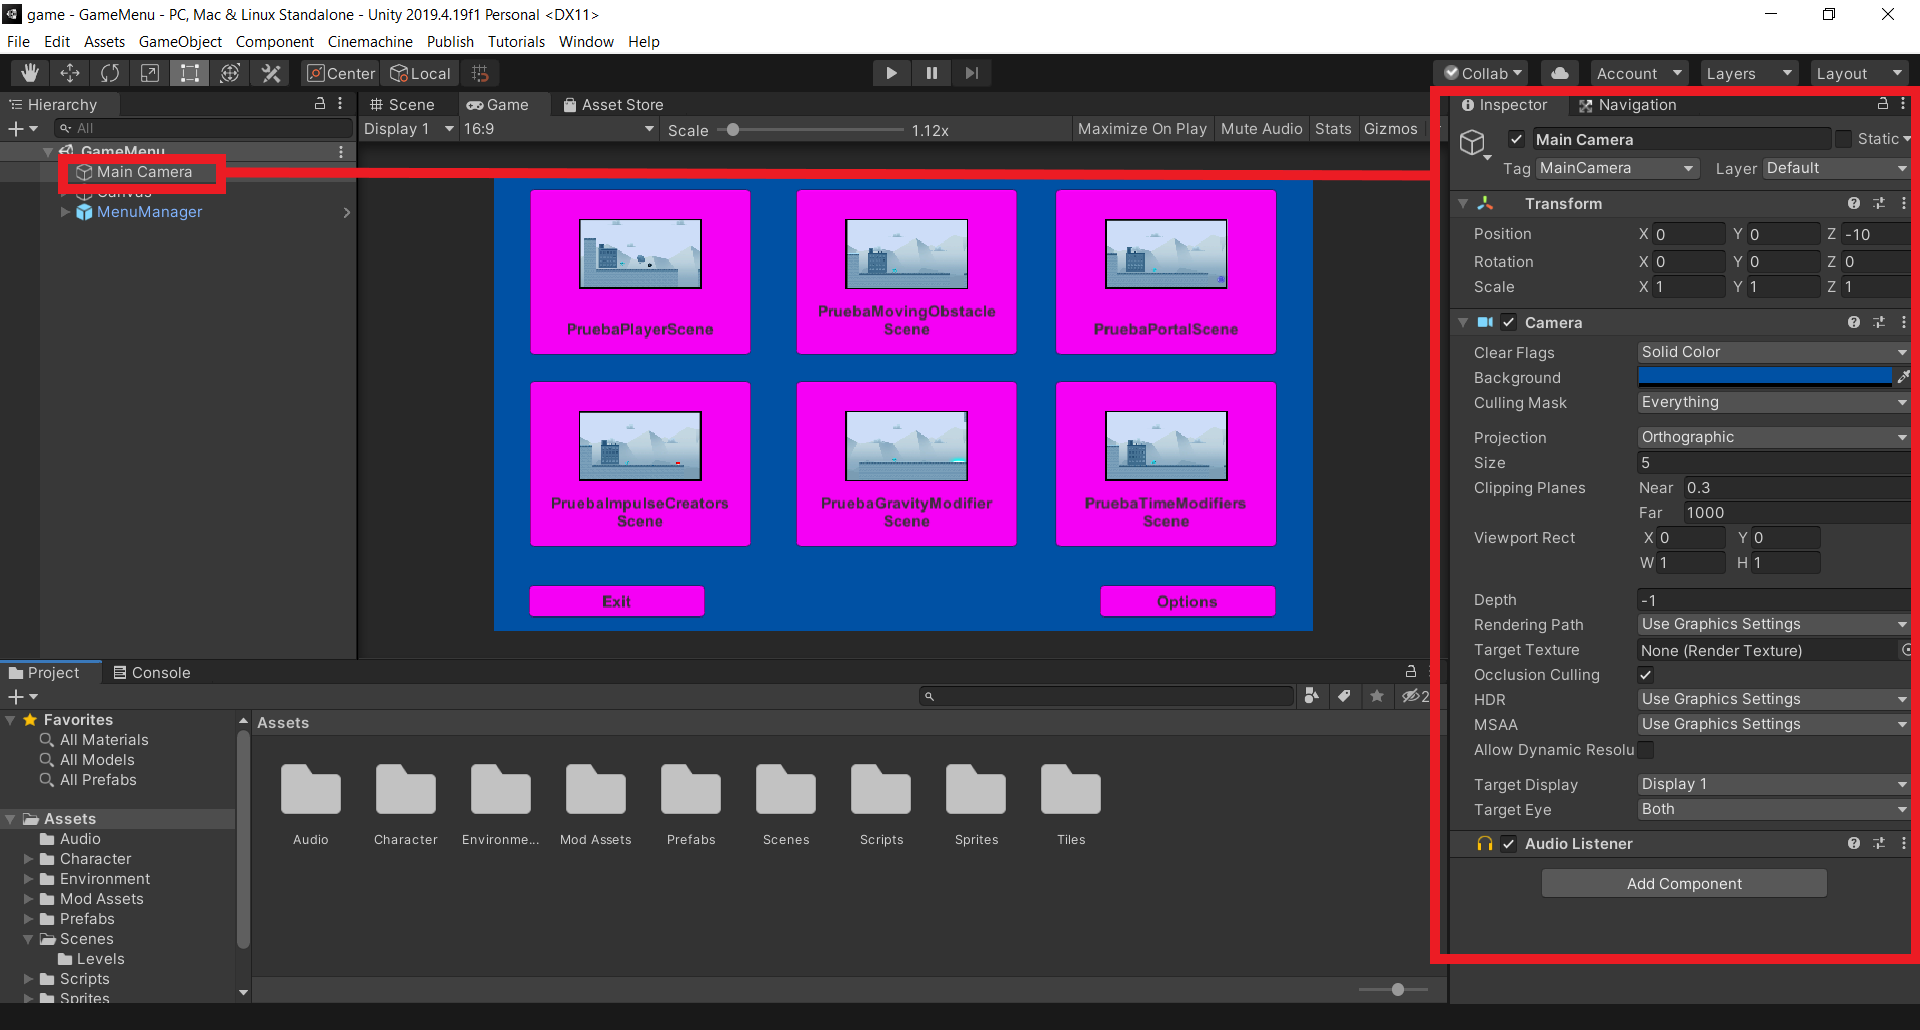
\includegraphics[scale=0.3]{Anexos/Anexo_D/Info}
\caption{Información asociada al GameObject Main Camera}
\end{figure}

\subsubsection{Game}
Ventana que muestra como se verá el juego en ejecución. Si se ejecuta el proyecto mostrará como se verá el juego en tiempo de ejecución actualizándose en cada frame.

\begin{figure}[h]
\centering
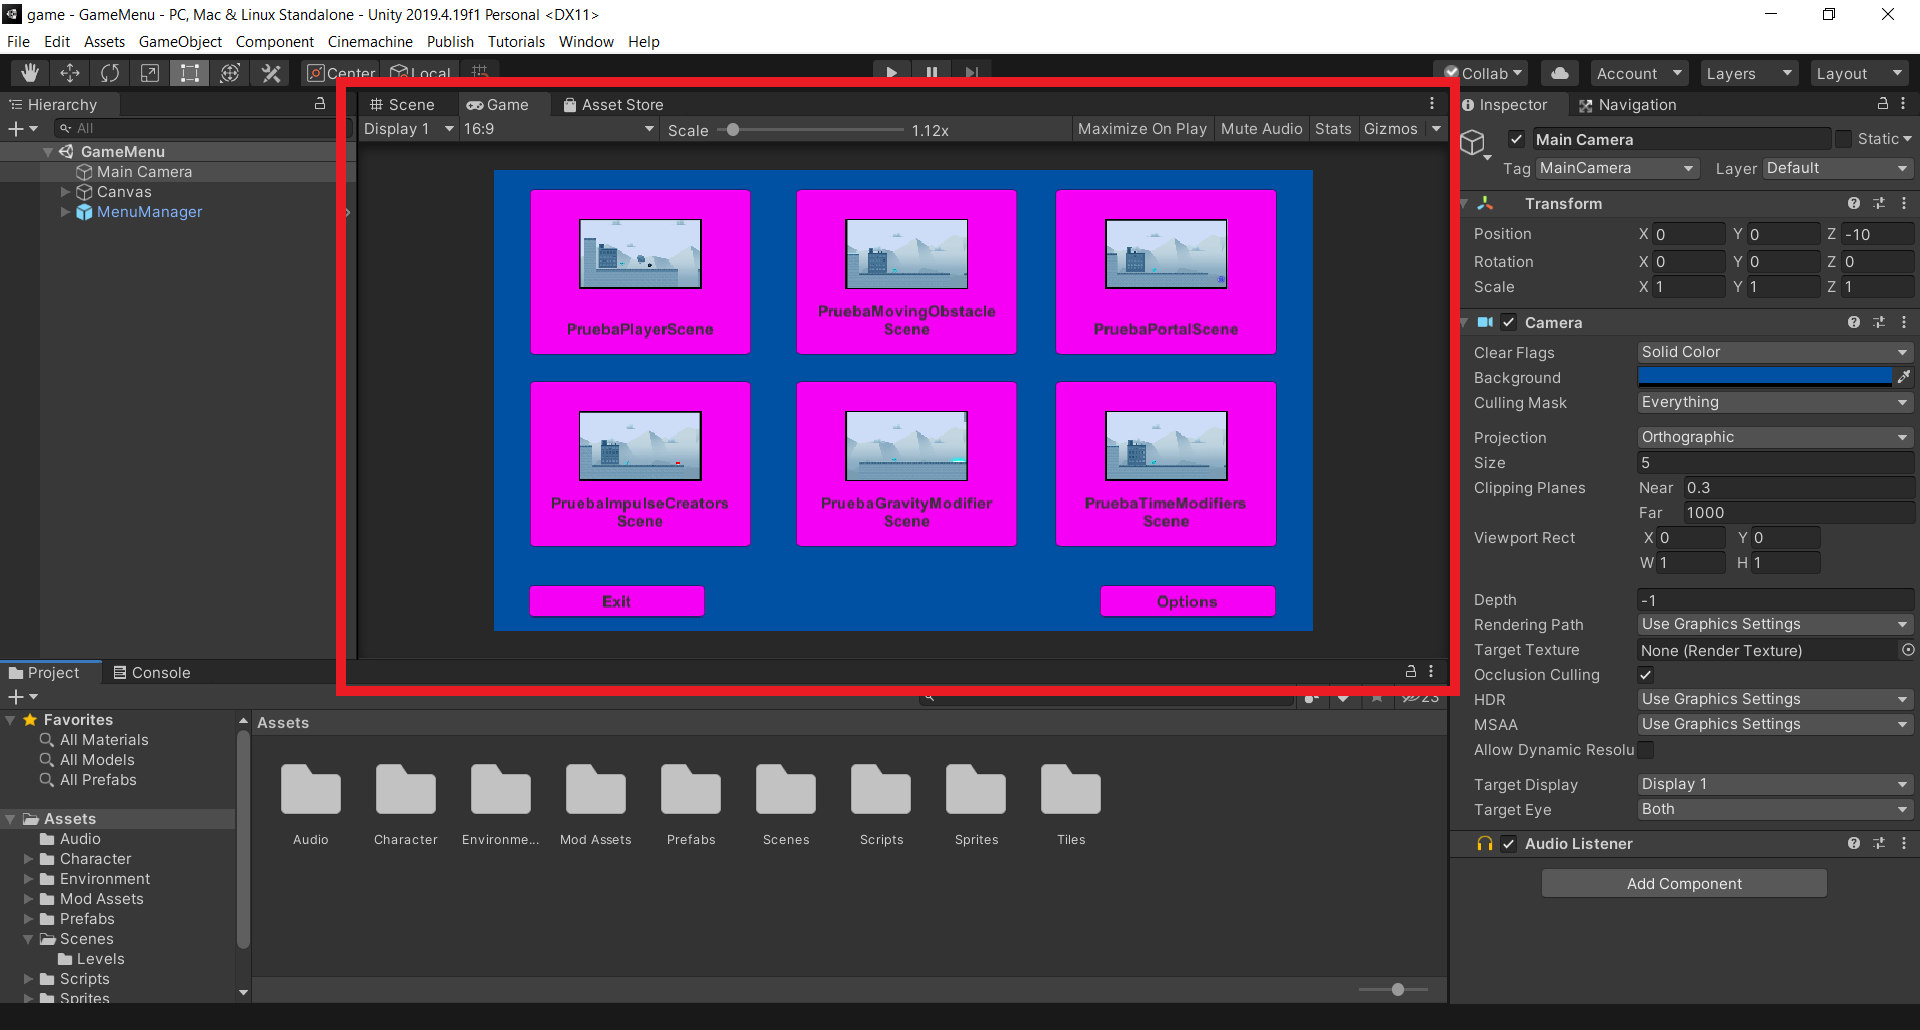
\includegraphics[scale=0.3]{Anexos/Anexo_D/Game}
\caption{Vetana ''Game'' de Unity}
\end{figure}

\subsubsection{Scene}
Ventana que muestra como visualmente donde estaría cada objeto de ''Hierarchy'' en un entorno físico. Como el desarrollo es de un Plataformas 2D se mostrará el entorno físico en dos dimensiones, pero también es posible generar el entorno en 3D (en realidad el entorno generado es 3D, pero con una colocación de cámara que simula ser 2D).

\clearpage
\begin{figure}[h]
\centering
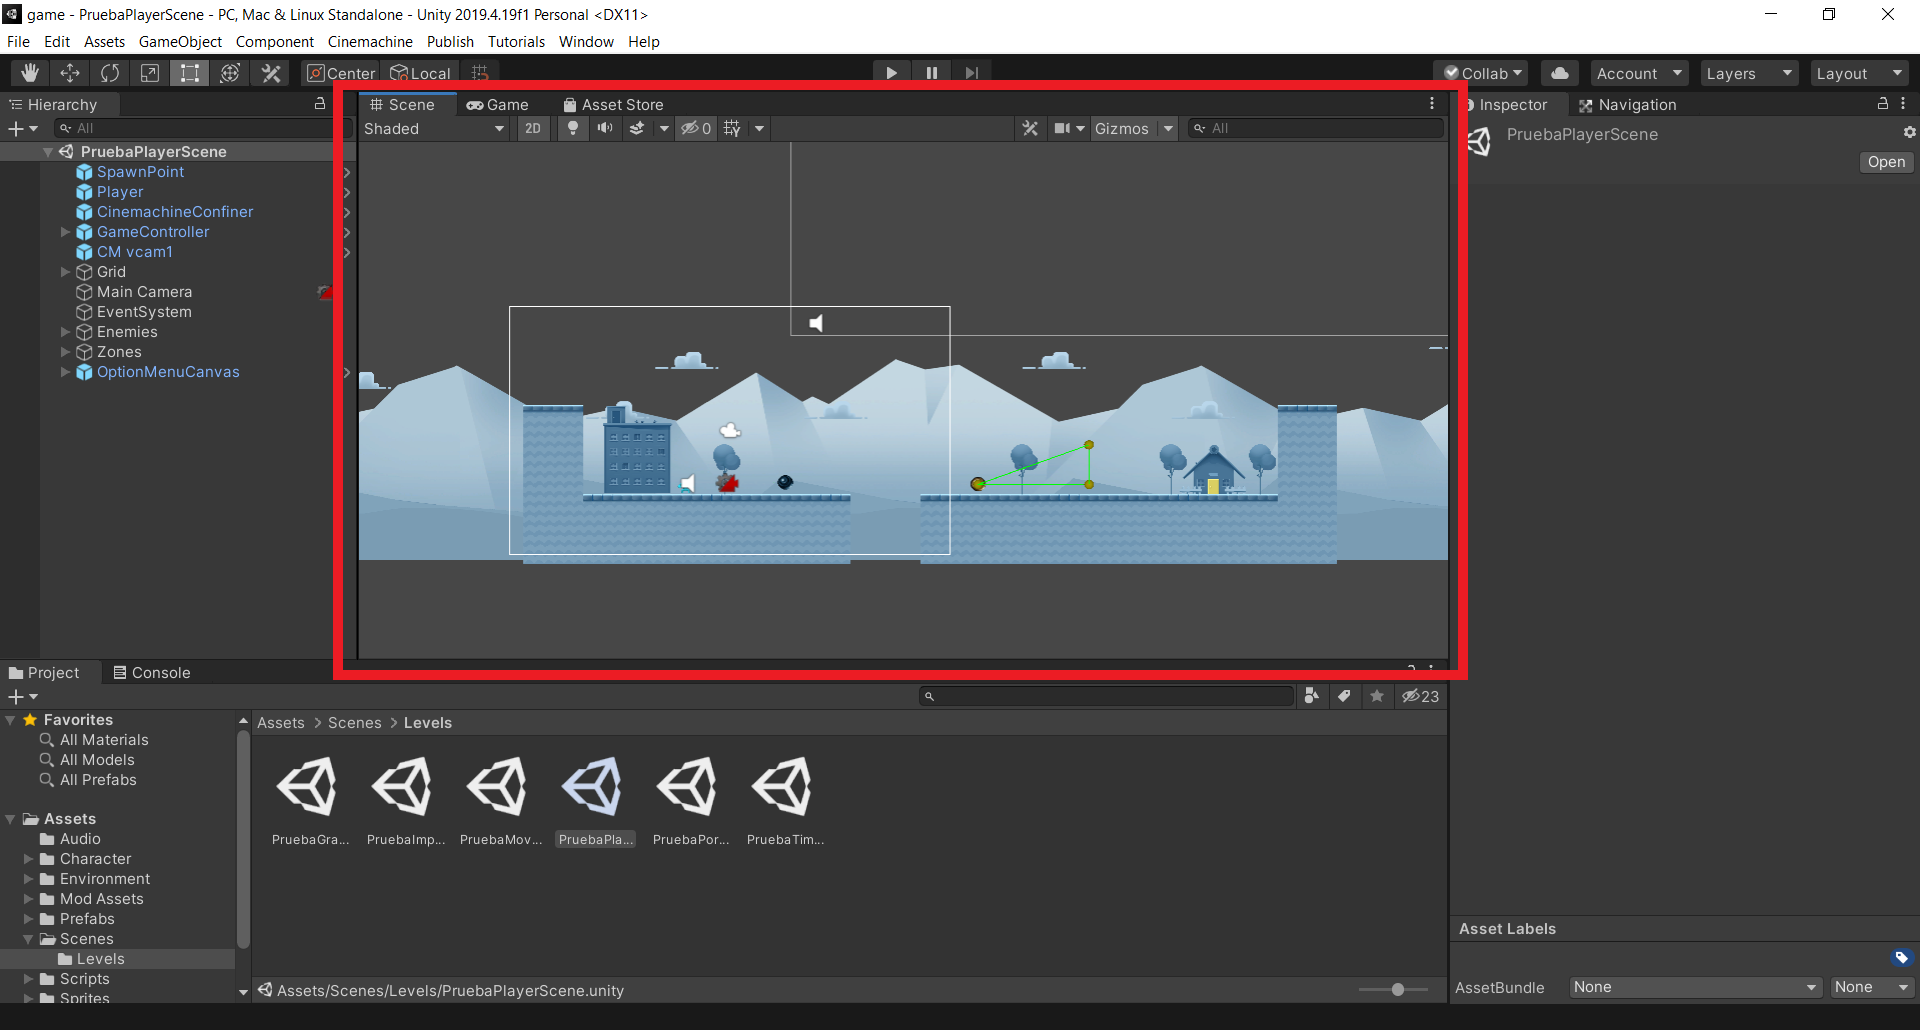
\includegraphics[scale=0.3]{Anexos/Anexo_D/Scene}
\caption{Ventana ''Scene'' de Unity}
\end{figure}

\subsection{Importación del proyecto}
El proyecto de Unity está en la carpeta game del repositorio de Github y será necesario guardado en el ordenador en el que se desee importar para poder importarlo.
Para importar el proyecto lo único que hay que hacer es, en el apartado ''Proyects'' del Unity Hub pulsar el botón de ''ADD''.

\begin{figure}[h]
\centering
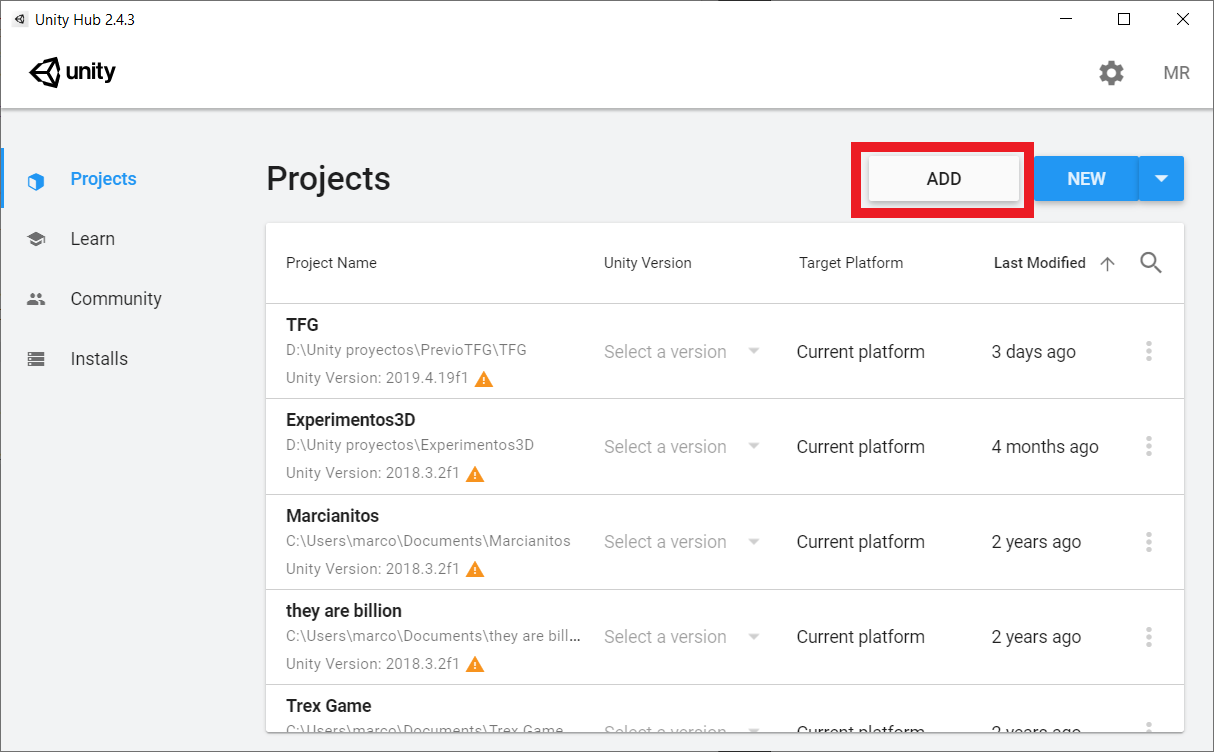
\includegraphics[scale=0.2]{Anexos/Anexo_D/Prujects_add}
\caption{Importación del proyecto de Unity desde Unity Hub}
\end{figure}
\clearpage

Después de pulsar el botón se pedirá una ruta. Introducir la ruta donde esté guardada la carpeta game del repositorio de GitHub.

\begin{figure}[h]
\centering
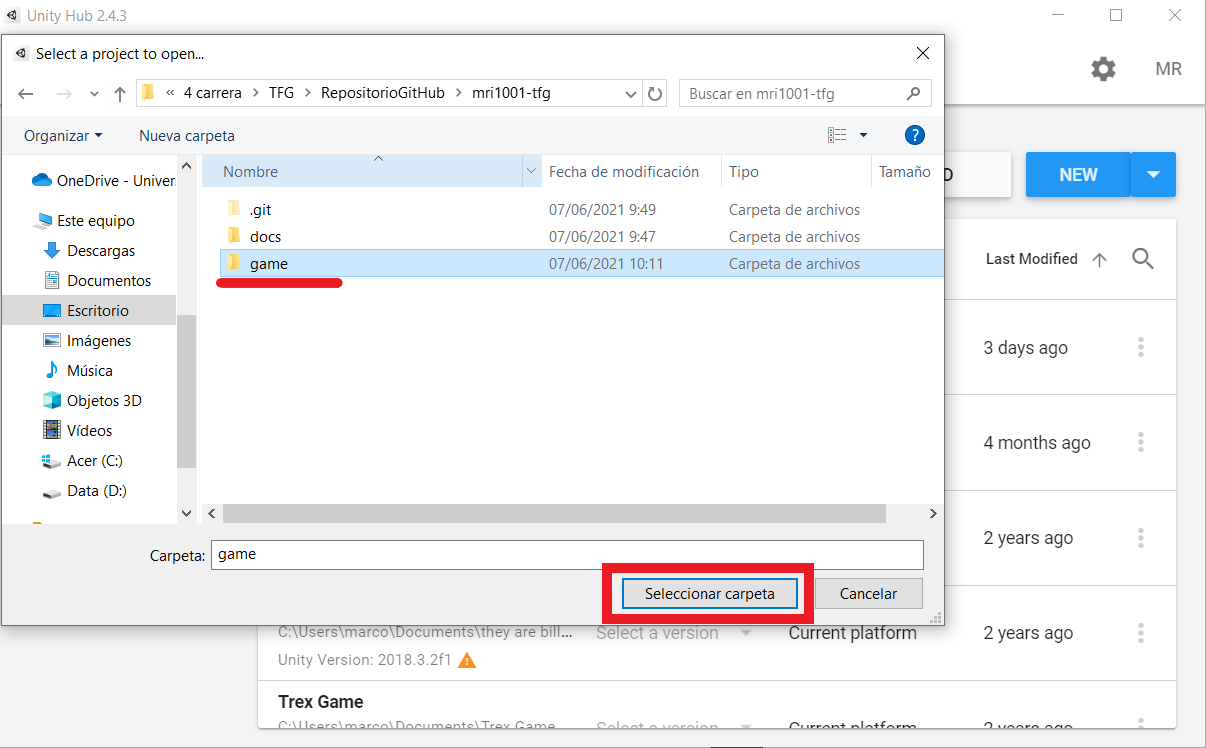
\includegraphics[scale=0.3]{Anexos/Anexo_D/Project_ruta}
\caption{Selección ruta del proyecto de Unity desde Unity Hub}
\end{figure}

Se añadirá a la lista de proyectos de Unity el proyecto importado y ya se podrá acceder a él.

\begin{figure}[h]
\centering
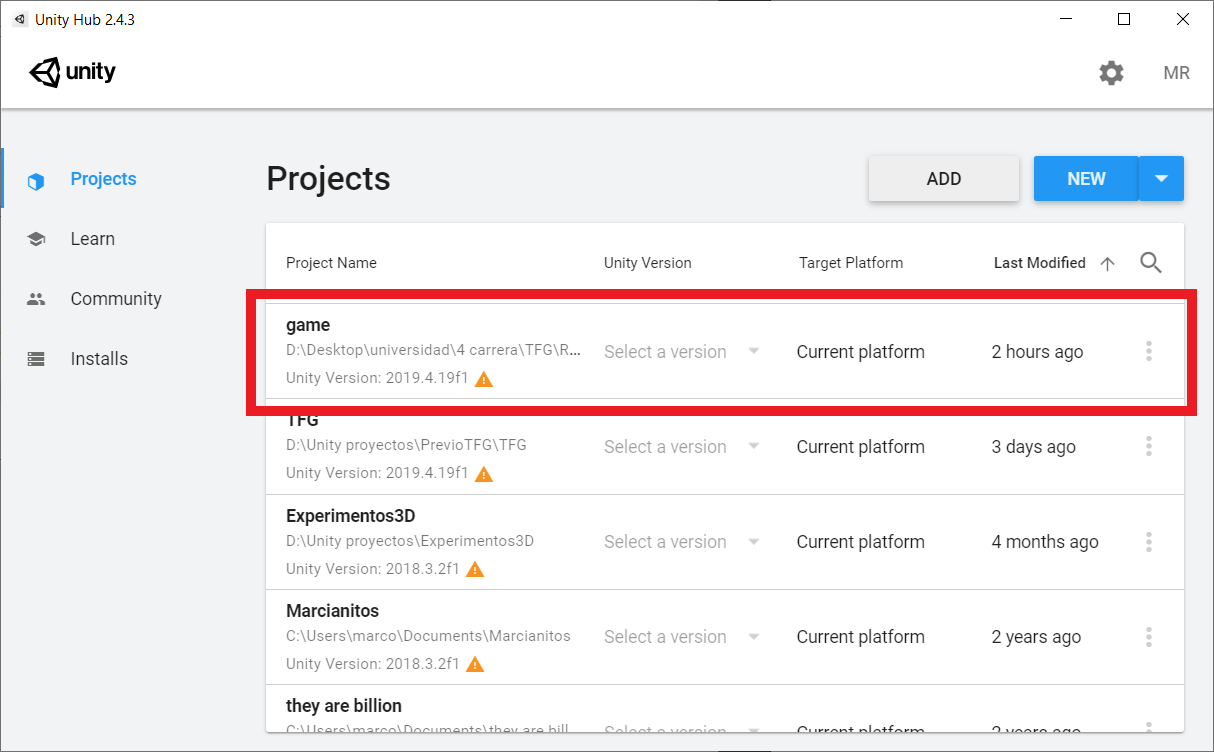
\includegraphics[scale=0.3]{Anexos/Anexo_D/Project_creado}
\caption{Proyecto importado correctamente}
\end{figure}

Al abrir el proyecto por primera vez saldrá una escena por defecto vacía. Con seleccionar cualquier otra escena será suficiente para que desaparezca esa escena y el funcionamiento sea el normal.

\subsection{Exportación del proyecto}
Para exportar el proyecto y generar el videojuego con su correspondiente ejecutable solo es necesario ir a la pestaña de File → Build Settings de la barra de herramientas superior del editor de Unity.\\
Al hacerlo aparecerá la siguiente ventana:

\begin{figure}[h]
\centering
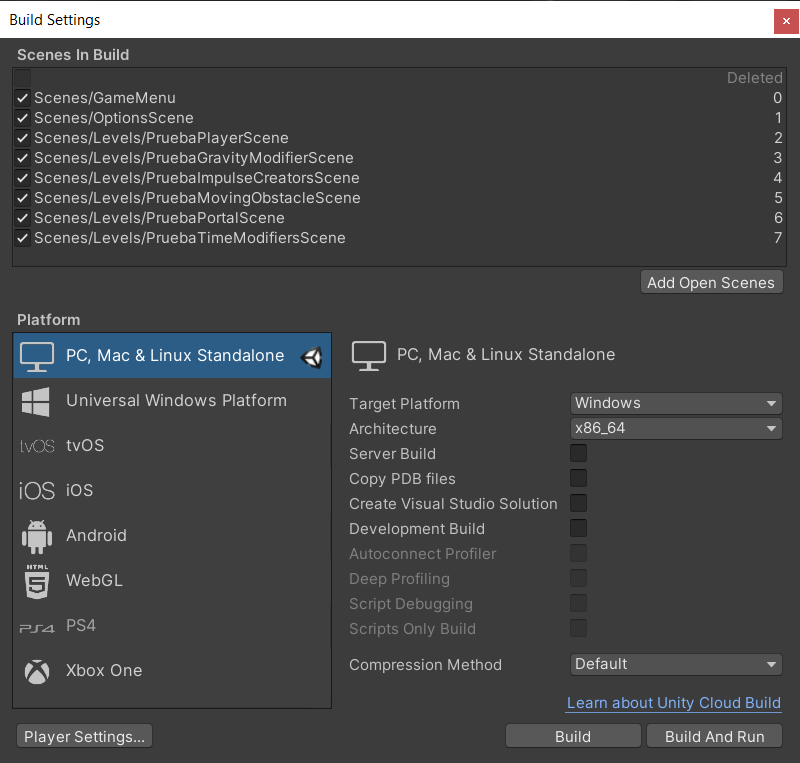
\includegraphics[scale=0.3]{Anexos/Anexo_D/Build}
\caption{Ventana de construcción del juego}
\end{figure}

Esta ventana da la opción de elegir a que sistema operativo y plataforma exportarlo entre otras opciones.

\begin{figure}[h]
\centering
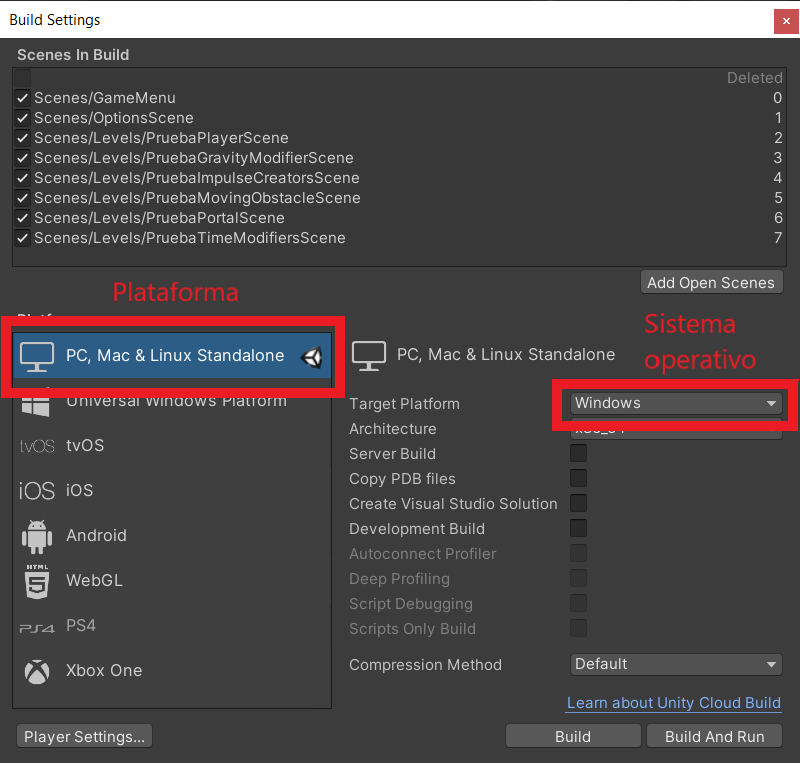
\includegraphics[scale=0.3]{Anexos/Anexo_D/Plataforma}
\caption{Seleción de plataforma y Sistema operativo}
\end{figure}

Es muy importante que el tick esté en todas las escenas a las que se desee transicionar para poder viajar a ellas.

\begin{figure}[h]
\centering
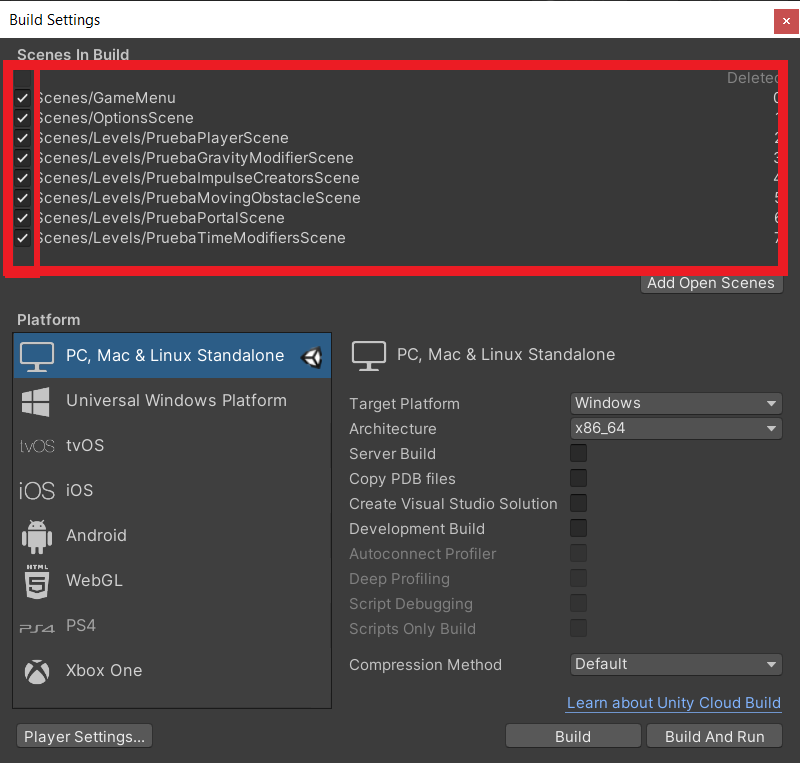
\includegraphics[scale=0.3]{Anexos/Anexo_D/Scenes}
\caption{Escenas seleccionadas para exportar}
\end{figure}

Una vez hecha esta comprobación se puede dar al botón ''Build'' para comenzar la exportación del juego. Pedirá una ruta para exportar el juego construido.

\begin{figure}[h]
\centering
\includegraphics[scale=0.3]{Anexos/Anexo_D/Export}
\caption{Ficheros generados al exportar el juego}
\end{figure}

Entre los ficheros generados un .exe. Ese es el que iniciará la ejecución del juego.

\section{Compilación, instalación y ejecución del proyecto}

\subsection{Instalación}
Para este proyecto solo es necesario tener instalado Unity. Para descargarlo hay que acceder a la siguiente página web: \url{https://unity3d.com/get-unity/download}

\begin{figure}[h]
\centering
\includegraphics[scale=0.3]{Anexos/Anexo_D/Descarga_Unity}
\caption{Página de descarga de Unity}
\end{figure}

Pulsando el botón de ''Download Unity Hub'' se descargará un ejecutable. Al ejecutarlo comenzará la instalación del Unity Hub. Es una instalación normal, con seguir las instrucciones y aceptar los términos de uso el Unity Hub se instalará correctamente.\\
Ahora solo falta descargar la versión de Unity que se desea. El proyecto se ha desarrollado en la versión de Unity 2019.4.19f1. Es importante tener cuidado con la versión a instalar, porque, es cierto que las versiones posteriores permiten importar el proyecto, pero si ha pasado mucho tiempo entre versiones algo se podría deprecado y no funcionar como se espera.

Para instalar La versión de Unity que queramos hay que abrir el Unity Hub y acceder a la pestaña ''Install''.

\clearpage
\begin{figure}[h]
\centering
\includegraphics[scale=0.3]{Anexos/Anexo_D/UnityHub}
\caption{Unity Hub}
\end{figure}

Una vez en esa pestaña pulsar el botón de add y elegir la versión de Unity que se desea descargar.

\begin{figure}[h]
\centering
\includegraphics[scale=0.3]{Anexos/Anexo_D/UnityHub_añadir}
\caption{Descarga de una versión de Unity desde Unity Hub}
\end{figure}

\clearpage
\begin{figure}[h]
\centering
\includegraphics[scale=0.3]{Anexos/Anexo_D/UnityHub_version}
\caption{Selección de una versión de Unity desde Unity Hub}
\end{figure}

Clicando en ''Next'' aparecerán los módulos de Unity que se desean añadir a la instalación. Añadir a los que se ofrecen por defecto los módulos ''Linux Build Support (IL2CPP)'' y ''Linux Build Support (Mono)'' para que al exportar el juego también sea compatible con Linux.

\begin{figure}[h]
\centering
\includegraphics[scale=0.3]{Anexos/Anexo_D/UnityHub_modulos}
\caption{Selección de módulos de Unity desde Unity Hub}
\end{figure}

Pulsar en ''Next'' y esperar a que termine la instalación.

La instalación también se puede llevar a cabo después de importar el proyecto, pues no te dejará abrir el proyecto y te obligará a realizar la instalación. El proceso es similar al mostrado anteriormente. Si no se sabe la versión de Unity del proyecto que se desea importar es recomendable utilizar esta opción y descargar la versión de Unity necesaria después de importar el proyecto.

\subsection{Compilación}
Unity se compila automáticamente. Cada vez que se modifiquen los scripts utilizados en el proyecto y se vuelva a la ventana de la aplicación de Unity se guardarán los cambios y compilará el proyecto. Si surgen errores se mostrarán en la consola que ofrece Unity.
 Adicionalmente la consola de Unity añade las opciones ''Clear'' para limpiar el contenido de la consola, ''Clear on Play'' para limpiar el contenido de la consola cada vez que se ejecute el juego en el editor, ''Collapse'' para juntar los mensajes de la consola que sean iguales en solo uno, ''Clear on Build'', para limpiar el contenido de la consola cada vez que se exporte el proyecto, y ''Error pause'' para pausar la ejecución del programa cuando salte un error de ejecución.

\begin{figure}[h]
\centering
\includegraphics[scale=0.3]{Anexos/Anexo_D/Consola_Unity}
\caption{Consola de Unity}
\end{figure}

Es posible que la consola no se encuentre en esa posición exacta de la ventana de Unity, pero siempre se podrá acceder a ella a través de la pestaña de Window → Windows → Console de la barra de herramientas superior de Unity.

\subsection{Ejecución del proyecto}
El proyecto se puede ejecutar antes de exportarlo para tener una aproximación a los que será el producto exportado. Para ello se ha de pulsar el botón de ''Play'' del editor de Unity. La ejecución se parará cuando se vuelva a pulsar el botón de ''Play''. Tener en cuenta que las instrucciones de cierre del programa no funcionarán en el editor pero si en la exportación.\\
La ejecución del programa se puede pausar desde el botón de ''Pause''. Cuando se vuelva a pulsar este botón se reanudará la ejecución.

\begin{figure}[h]
\centering
\includegraphics[scale=0.3]{Anexos/Anexo_D/Play_Pause}
\caption{Botones de ''Play'' y ''Pause'' del editor de Unity}
\end{figure}

\section{Pruebas del sistema}
Como se ha mencionado en la memoria la realización de pruebas durante el desarrollo de un videojuego es un tema complejo. Debido a ello no ha sido posible realizar pruebas automáticas. Sin embargo, se ha querido representar el funcionamiento básico de videojuego (deducido a partir de los casos de uso y el documento de diseño de juego), que si bien no sirven como sistema de pruebas, formalizan el funcionamiento esperado del programa, permitiendo comprobar si se está realizando una correcta implementación del programa o allanando en el terreno por si en el futuro fuese posible implementar pruebas automáticas.

Para este propósito se ha seguido el sistema de representación de test Given-When-Then \cite{GWT}. Este sistema de representación se sirve de tres premisas para estructurar los test:
\begin{itemize}
\item
Given: Para describir el estado del programa antes de realizar la acción que se desea probar.
\item
When: Representará la acción que se desea probar.
\item
Then: Para describir los cambios esperados tras la realización de la prueba a realizada.
\end{itemize}

Se mostrarán a continuación las representaciones de los test desarrolladas:

\subsection{Selección de niveles}
\textbf{Given:} Se está en el menú principal.

\textbf{When:} Se selecciona el nivel al que se desea viajar (PruebaPlayerScene) y se pulsa el botón de acceso.

\textbf{Then:} Se ha viajado a la escena del nivel seleccionado (PruebaPlayerScene)

\subsection{Viaje al menú de opciones}
\textbf{Given:} Se está en el menú principal.

\textbf{When:} Se selecciona el botón de Options y se pulsa.

\textbf{Then:} Se ha viajado al menú de opciones (OptionsScene)

\subsection{Modificar una opción}
\textbf{Given:} Se está en el menú principal sobre la opción de Volumen general, que tiene el valor de 100.

\textbf{When:} Mover la barra de desplazamiento lo máximo hacia la izquierda.

\textbf{Then:} El texto que marca el valor del volumen general habrá cambiado a 0. El volumen del juego será 0. Si se para la aplicación y se vuelve a correr el volumen general seguirá siendo 0.

\subsection{Abrir el menú de pausa}
\textbf{Given:} Estar en un nivel jugable (PruebaPlayerScene).

\textbf{When:} Pulsar el botón asociado a la apertura del menú de pausa.

\textbf{Then:} Se ha abierto el menú de pausa y la ejecución del nivel se habrá detenido temporalmente (Time.timeScale será 0).

\subsection{Cerrar el menú de pausa}
\textbf{Given:} Estar en un nivel jugable (PruebaPlayerScene) con el menú de opciones abierto.

\textbf{When:} Se pulsará el botón del controlador que se esté usando asociado al cierre del menú de pausa o se pulsará el botón del menú de pausa asociado con el cierre del menú de pausa.

\textbf{Then:} Se ha cerrado el menú de pausa y la ejecución del nivel se habrá retomado (Time.timeScale será 1).

\subsection{Vuelta al menú principal}
\textbf{Given:} Estar en un nivel jugable (PruebaPlayerScene) con el menú de opciones abierto.

\textbf{When:} Pulsar el botón del menú de opciones ''Back to Main Menú''.

\textbf{Then:} Se habrá pasado al menú principal.

\subsection{Invertir gravedad del Player}
\textbf{Given:} Estar en un nivel jugable con inversores de gravedad (PruebaGravityModifiersScene). El Player tiene una gravedad de Phisics2d.gravity (sin modificaciones).

\textbf{When:} El Player entra en contacto con un inversor de gravedad.

\textbf{Then:} La gravedad del Player se invierte siendo ahora -Phisics2d.gravity.

\subsection{Entrar a la zona de influencia de un obstáculo superdenso}
\textbf{Given:} Estar en un nivel jugable con un obstáculo superdenso (PruebaGravityModifiersScene). El Player tiene una gravedad de Phisics2d.gravity (sin modificaciones).

\textbf{When:} El Player entra en la zona de influencia del obstáculo superdenso.

\textbf{Then:} La gravedad del Player se modifica al entrar en la zona de influencia, aumentando en la dirección del obstáculo superdenso hasta que colisiona con este y muere.

\subsection{Entrar en una zona de modificación temporal}
\textbf{Given:} Estar en un nivel jugable con una zona de modificación temporal (PruebaTimeModifiersScene). La escala de tiempo del Player es la por defecto.

\textbf{When:} El Player se desplaza hasta entrar en la zona de modificación temporal.

\textbf{Then:} La escala de tiempo del Player pasa a ser la escala de tiempo por defecto * la modificación a la escala temporal de la zona de modificación temporal.

\subsection{Salir de una zona de modificación temporal}
\textbf{Given:} Estar en un nivel jugable con una zona de modificación temporal (PruebaTimeModifiersScene). El Player se encuentra en una zona de modificación temporal. La escala de tiempo del Player es la por defecto * la modificación a la escala temporal de la zona de modificación temporal.

\textbf{When:} El Player se desplaza hasta salir de la zona de tiempo invertido.

\textbf{Then:} La escala de tiempo del Player pasa a ser la escala que tenía / la modificación a la escala temporal de la zona de modificación temporal (la escala de tiempo por defecto).

\subsection{Modificar el tiempo a nivel global}
\textbf{Given:} Estar en un nivel jugable (PruebaPlayerScene).

\textbf{When:} Pulsar el botón asociado a la mecánica de tiempo bala del Player.

\textbf{Then:} La ejecución del nivel se reducirá (Time.timescale se reducirá) y pasado un tiempo volverá a su estado natural (Time.timescale = 1)

\subsection{Utilizar una plataforma de salto}
\textbf{Given:} Estar en un nivel jugable con una plataforma de salto (PruebaImpulseCreatorsScene).

\textbf{When:} El Player entra en contacto con la plataforma de salto.

\textbf{Then:} El Player sale impulsado hacia arriba. Su velocidad (la RigidBody2D.Velocity del Player) habrá variado en el eje de las Y, pero no en el de las X. RigidBody2D.Velocity.Y del Player será ahora RigidBody2D.Velocity.Y + impulso de la plataforma de salto. RigidBody2D.Velocity.X deberá seguir siendo la misma.

\subsection{Utilizar una partícula de impulso}
\textbf{Given:} Estar en un nivel jugable con una partícula de impulso (PruebaImpulseCreatorsScene).

\textbf{When:} El Player entra en contacto con la partícula de impulso.

\textbf{Then:} El Player sale impulsado en la dirección designada por la partícula de impulso. RigidBody2D.Velocity.Y del Player será ahora RigidBody2D.Velocity.Y + impulso de la partícula de impulso en el eje de las Y. RigidBody2D.Velocity.X deberá ser RigidBody2D.Velocity.X + impulso de la partícula de impulso en el eje de las X.

\subsection{Utilizar un amplificador de impulso}
\textbf{Given:} Estar en un nivel jugable con un amplificador de impulso (PruebaImpulseCreatorsScene).

\textbf{When:} El Player entra en contacto con el amplificador de impulso.

\textbf{Then:} La velocidad del Player se escalará en la cantidad designada por el amplificador de impulso. RigidBody2D.Velocity del Player será ahora RigidBody2D.Velocity * multiplicador del amplificador de impulso.

\subsection{Colisionar con una pared}
\textbf{Given:} Estar en un nivel jugable con paredes (PruebaPlayerScene). El Player lleva una velocidad de 6 en el eje de las X y -3 en el de las Y.

\textbf{When:} El Player colisiona con una pared a su derecha (la dirección en el eje de las X en el que se está desplazando).

\textbf{Then:} El Player debe estar al lado de la pared. La velocidad en la dirección del muro debe cesar pero el resto continuar. La velocidad del Player será ahora 0 en el eje de las X y -3 en el eje de las Y.

\subsection{Colisionar con el suelo}
\textbf{Given:} Estar en un nivel jugable con suelos (PruebaPlayerScene). El Player lleva una velocidad de 6 en el eje de las X y -3 en el de las Y.

\textbf{When:} El Player colisiona con el suelo que hay a sus pies (la dirección en el eje de las Y en el que se está desplazando).

\textbf{Then:} El Player debe estar encima del suelo. La velocidad en la dirección del suelo debe cesar pero el resto continuar. La velocidad del Player será ahora 6 en el eje de las X y 0 en el eje de las Y.

\subsection{Entrar por un portal}
\textbf{Given:} Estar en un nivel jugable con un par de portales enlazados (portal1 y portal2) (PruebaPortalesScene).

\textbf{When:} El Player entra por el portal1.

\textbf{Then:} El Player se habrá teletransportando pasando a ser su nueva posición la del portal2.

\subsection{Mover al Player a la derecha}
\textbf{Given:} Estar en un nivel jugable con un Player (PruebaPlayerScene).

\textbf{When:} El Player pulsa el botón de desplazamiento hacia la derecha.

\textbf{Then:} La velocidad del Player habrá aumentado en el eje de las X positivamente. El Player se habrá desplazado hacia la derecha.

\subsection{Mover al Player a la izquierda}
\textbf{Given:} Estar en un nivel jugable con un Player (PruebaPlayerScene).

\textbf{When:} El Player pulsa el botón de desplazamiento hacia la izquierda.

\textbf{Then:} La velocidad del Player habrá disminuido en el eje de las X. El Player se habrá desplazado hacia la izquierda.

\subsection{Saltar con el Player}
\textbf{Given:} Estar en un nivel jugable con un Player (PruebaPlayerScene).

\textbf{When:} El Player pulsa el botón de salto.

\textbf{Then:} La velocidad del Player habrá aumentado en el eje de las Y. El Player realizará el salto.

\subsection{Realizar el acelerón con el Player}
\textbf{Given:} Estar en un nivel jugable con un Player (PruebaPlayerScene).

\textbf{When:} El Player pulsa el botón del acelerón.

\textbf{Then:} La velocidad del Player pasará a ser constante siendo 0 en el eje de las Y, y +(velocidad del aceleron) en el eje de las X en caso de haber estado yendo hacia la derecha o -(velocidad del aceleron) en el eje de las X en caso de haber estado yendo hacia la izquierda. El Player realizará el salto.

\subsection{Muerte contra un obstáculo}
\textbf{Given:} Estar en un nivel jugable con obstáculos (PruebaPlayerScene).

\textbf{When:} El Player colisiona con el obstáculo.

\textbf{Then:} Se debe iniciar la cadena de eventos de muerte del Player.

\subsection{Cadena de eventos de la muerte del Player}
\textbf{Given:}Estar en un nivel jugable (PruebaPlayerScene).

\textbf{When:} El Player muere.

\textbf{Then:} Se destruyen los objetos instanciados durante la ejecución el nivel y se reinicia el nivel devolviéndolo al estado inicial.

\subsection{El Player cae en una zona de muerte}
\textbf{Given:} Estar en un nivel jugable con zonas de muerte (PruebaPlayerScene).

\textbf{When:} El Player colisiona con la zona de muerte.

\textbf{Then:} Se debe iniciar la cadena de eventos de muerte del Player.

\subsection{El Player cae en una zona de victoria}
\textbf{Given:} Estar en un nivel jugable con zonas de victoria (PruebaPlayerScene).

\textbf{When:} El Player colisiona con la zona de victoria.

\textbf{Then:} El Player realiza la animación de llegada a la zona de victoria y se transiciona al menú principal.

\subsection{El obstáculo que sigue una rutina se mueve}
\textbf{Given:} Estar en un nivel jugable con un obstáculo que sigue una rutina (PruebaPlayerScene).

\textbf{When:} Pasar loops de ejecución del programa.

\textbf{Then:} El obstáculo debe haber pasado por todos los puntos que componen su rutina de viaje y haber vuelto a la posición inicial. Al haber vuelto a la posición inicial se debe continuar el movimiento del obstáculo repitiendo la rutina del viaje hasta que se pare la ejecución.

\subsection{El obstáculo móvil se mueve}
\textbf{Given:} Estar en un nivel jugable con un obstáculo que sigue una rutina (PruebaMovingObstacleScene).

\textbf{When:} Pasar loops de ejecución del programa.

\textbf{Then:} El obstáculo móvil tiene que avanzar de derecha a izquierda indefinidamente. Su posición en el eje de las X tiene que ser siempre menor que la que llevaba anteriormente.
\apendice{Documentación de usuario}

\section{Introducción}
Puede ser que el usuario tenga dudas sobre el producto entregado o el manejo de este. En este anexo se ofrecerá toda la información que el usuario puede requerir para hacer un uso adecuado del producto entregado.

\section{Requisitos de usuarios}
El único requisito para que el usuario pueda ejecutar el videojuego es tener un ordenador con un sistema operativo Windows o Linux.

La otra preocupación del usuario puede ser que su ordenador no sea capaz de correr el juego debido a que es demasiado exigente. Es cierto que esto puede ocurrir con algunos juegos, pero suelen ser juegos de proporciones titánicas, con muchos eventos ocurriendo simultáneamente y con gráficos mucho más sofisticados que los de este juego.\\
A pesar de que se tiene la firme creencia firme de que puede ejecutar en prácticamente cualquier ordenador se van a listar las especificaciones de los dos ordenadores sobre los que se ha ejecutado el juego y comprobado su correcto funcionamiento.

\subsection{Predator PH315-51}
\begin{itemize}
\item
Procesador Intel Core i7-8750H (6 núcleos, 9 MB Caché, 2.2 GHz hasta 4.1 GHz)
\item
Memoria RAM de 16 GB DDR4 (alcanzando un pico de 141MB cuando se ejecuta)
\item
Disco HDD de 1 TB
\item
Disco SSD de 128 GB
\item
Tarjeta gráfica Nvidia GeForce GTX 1060
\item
Sistema operativo Windows 10 Home
\end{itemize}

\subsection{Ordenador de ofimática}
\begin{itemize}
\item
Procesador Intel Core i3-6006U (6 núcleos, 9 MB Caché, 2 GHz)
\item
Memoria RAM de 4 GB DDR4
\item
Disco SSD de 200 GB
\item
Tarjeta gráfica Intel HD Graphics 520 (integrada)
\item
Sistema operativo Windows 10 Home
\end{itemize}

En ambos ordenadores el videojuego funciona sin ralentizaciones ni caídas de frames. Es cierto, aun así, que el ordenador de ofimática tarda un par de segundos más en cambiar entre escenas más que el otro ordenador (mucho más potente).

\subsection{Linux}
Para sistemas operativos Linux se ha ejecutado el juego en un ordenador con las siguientes especificaciones:
\begin{itemize}
\item
Procesador Intel(R) Core(TM) i3-5005U CPU @ 2.00GHz (4 núcleos)
\item
Memoria 8GB (usando algo menos de 116MB cuando se ejecuta)
\item
Tarjeta gráfica Intel HD Graphics 5500 (integrada)
\item
Sistema operativo Ubuntu 20.04.1
\end{itemize}

\subsection{Requisitos mínimos}
Partiendo de las pruebas hechas se puede generar un listado de recursos mínimos que consumirá la ejecución del videojuego:
\begin{itemize}
\item
130 MB de disco duro los ficheros que contienen el juego (en la versión de Linux que es la que más ocupa)
\item
150 MB de RAM
\item
Un 8\% de la CPU
\item
Un 17\% de la GPU
\end{itemize}

\section{Instalación}
El usuario no tendrá que instalar nada para poder iniciar el videojuego. Bastará con que se descargue el contenido del repositorio de GitHub asociado al proyecto (\url{https://github.com/Kencho/mri1001-tfg}).

Una vez descargado el repositorio, dentro de la carpeta executables, habrá tres ficheros comprimidos (game\_Windows.zip, game\_Linux.tar.gz y game\_WebGL.zip) que contendrán la estructura de ficheros del videojuego y el ejecutable que permitirá iniciarlo.

El usuario solo tendrá que descomprimir el fichero asociado a su sistema operativo o el fichero de WebGL si no se quiere estar atado a ningún sistema operativo. Después tendrá que entrar en la carpeta generada y ejecutar el fichero .exe. Esto iniciará la ejecución del videojuego.

\subsection{Instalación WebGL}
Sin embargo, es importante mencionar que para la versión de WebGL es necesario que el buscador con el que lo abres soporte WebGL. Esto se pude comprobar accediendo al siguiente enlace: \url{https://get.webgl.org/}.\\ 
Al entrar en esta página hay dos opciones: visualizar un cubo rotando o no visualizarlo. Si se visualiza significa que el navegador soporta WebGL.\\
Lo más probable es que cualquier navegador moderno popular que utilices soporten WebGL. Aun así, se ha comprobado empíricamente que los siguientes navegadores soportan WebGL:
\begin{itemize}
\item
Google Chrome
\item
Mozilla Firefox
\item
Microsoft Edge
\item
Internet Explore
\item
Opera
\end{itemize}

En caso de que no se vea el cubo rotando, lo más probable es que con actualizar los Drivers de la tarjeta gráfica se solucione el problema.

\clearpage
\begin{figure}[h]
\centering
\includegraphics[scale=0.65]{Anexos/Anexo_E/Cubo_WebGL}
\caption{Cubo que rota si el navegador soporta WebGL}
\end{figure}

Aunque el navegador soporte WebGL, es muy probable que al ejecutar el fichero .html que inicia la ejecución en WebGL salte un error.

\begin{figure}[h]
\centering
\includegraphics[scale=0.65]{Anexos/Anexo_E/Error_WebGL}
\caption{Error de la versión del ejecutable de WebGL}
\end{figure}

Este error no es realmente un error, sino una restricción de permisos. Los navegadores suelen tener una opción de seguridad que impide a las páginas acceder a recursos file://. Sin esta restricción se podría acceder a los ficheros del equipo, lo cual es una gran riesgo.\\
Para poder ejecutar el juego en WebGL sin hacer uso de un servidor web es necesario desactivar esta opción. Esta opción se puede desactivar siguiendo los pasos de explicados en el siguiente enlace: \url{https://bit.ly/3iEMWAj}.\\
Esta versión del ejecutable no es recomendable que un usuario que solo quiera disfrutar del videojuego la use. Ha sido añadida como opción para el desarrollo, esperando que se aloje en un servidor web.

\section{Manual del usuario}
Bienvenido, \textit{\textbf{JUGADOR}}, a nuestro nuevo videojuego. Ha habido un \textcolor{endeavour}{cataclismo intergaláctico} y los \textcolor{azulWorker}{ciber trabajadores espaciales} se han extraviado de camino a sus oficinas.


¿Serán capaces de volver los \textcolor{azulWorker}{ciber trabajadores} a la oficina para que puedan generar beneficios a la empresa antes de que se vuelvan un lastre y los despidan?

Se trata de un Plataformas 2D dónde podrá controlar a los \textcolor{azulWorker}{ciber trabajadores} y hacer uso de todas las herramientas de modificación del espacio y el tiempo que les provee su generoso jefe para recorrer el \textcolor{endeavour}{espacio multidimensional}.\\
Pero cuidado, muchos son los peligros que les aguardan y extraño el camino que ahora lleva hasta las oficinas.

\subsection{Controles}
Al iniciar el juego se encontrará con el menú principal. Desde él podrá seleccionar que \textcolor{azulWorker}{trabajador} desea ayudar a llegar a la oficina (como el 30 veces consecutivas empleado del mes, PruebaPlayerScene, o el irreemplazable conserje PruebaMovingObstacleScene).

¡Seleccione a que \textcolor{azulWorker}{trabajador} desea ayudar y tome posesión de su cuerpo para asegurarse de que no le despidan!

Pero igual no esta muy ducho en el arte de poseer \textcolor{azulWorker}{trabajadores}, o incluso de navegar por los abstractos \textit{"""Menús del juego"""}, que por supuesto no existen en otro \textcolor{endeavour}{plano astral} completamente distinto al de los \textcolor{azulWorker}{trabajadores}.

No pasa nada, \textit{\textbf{JUGADOR}}, vallamos paso a paso.

\subsubsection{Controles del menú principal}
Para navegar por los menús del juego solo tendrá que tener claro que botón esta seleccionado ahora mismo. Eso lo sabrá por que, a diferencia del resto de botones, de color \textcolor{fucsia}{rosa fucsia}, el botón seleccionado será de color \textcolor{flirk}{rosa flirt}.

Ahora que usted,  \textit{\textbf{JUGADOR}}, sabe en que botón se encuentra solo necesita saber que acciones puede realizar desde él.
\begin{itemize}
\item
Podrá ir al rescate accediendo al nivel jugable pulsando el botón "X" de su mando (entendemos está usando una mando de Play Station) o la tecla "ENTER" de su teclado. En cuanto lo haga viajará al \textcolor{endeavour}{esperpéntico mundo} en el que el \textcolor{azulWorker}{trabajador} espera a ser devuelto a su oficina.
\item
Si le cae mal ese \textcolor{azulWorker}{trabajador} en particular y desea salvar a otro, podrá desplazarse al botón en el que se encuentra su \textcolor{azulWorker}{\textbf{trabajador favorito}} y acudir en su rescate.\\
De un botón se podrá viajar a otro de la siguiente manera:
\begin{itemize}
\item
Si desea desplazarse al botón que se encuentra sobre el botón seleccionado empuje el Stick izquierdo del mando hacia arriba o pulse la flecha que apunta hacia arriba del teclado.
\item
Si, en cambio, desea desplazarse al botón que se encuentra bajo el botón seleccionado empuje el Stick izquierdo del mando hacia abajo o pulse la flecha que apunta hacia abajo del teclado.
\item
Si el desplazamiento vertical entre botones lo tiene dominado pruebe a  desplazarse al botón que se encuentra a la derecha del botón seleccionado. Empuje el Stick izquierdo del mando hacia la derecha o pulse la flecha que apunta hacia la derecha del teclado.
\item
Quiza le parezca, \textit{\textbf{JUGADOR}}, una decisión de diseño arriesgada, pero si desea desplazarse al botón que se encuentra a la izquierda del botón seleccionado empuje el Stick izquierdo del mando hacia la izquierda o pulse la flecha que apunta hacia la izquierda del teclado.
\end{itemize}
\item
Es posible que la misteriosa música que ha invadido el universo (o todo sonido en general) le resulte molesta. Viaje al menú de opciones y cambie asignele el valor que desee al volumen. Puede acceder al menú de opciones seleccionando el boton "Options".
\item
Si esta cansado de los \textcolor{azulWorker}{trabajadores} se aprovechen de tu buena fe para llegar al trabajo sin dar palo al agua y desea abandonarles a su suerte, no pasa nada. Cierre el juego pulsando el botón de "Exit" y tómese unas merecidas vacaciones que se descontarán de su sueldo.\\
Pero ¡cuidado!, es posible que los \textcolor{azulWorker}{trabajadores} sigan en su sitio a la espera de ser rescatados cuando vuelva a abrir el juego.
\end{itemize}

\begin{figure}[h]
\centering
\includegraphics[scale=0.65]{Anexos/Anexo_E/Mando_menus}
\caption{Controles de mando del menú}
\end{figure}

\begin{figure}[h]
\centering
\includegraphics[scale=0.65]{Anexos/Anexo_E/Teclado_menus}
\caption{Controles de teclado del menú}
\end{figure}

\subsubsection{Menú de pausa}
Se encuentra, \textit{\textbf{JUGADOR}}, en el menú de pausa. Desde este menú podrá modificar el volumen general situándose sobre la barra de desplazamiento de "General Volume" (de la misma forma que se hace con los botones del manú principal).\\
Empujando el Stick izquierdo del mando hacia la derecha o pulsando la flecha que apunta hacia la derecha del teclado se aumentará el volumen general.\\
Empujando el Stick izquierdo del mando hacia la izquierda o pulsando la flecha que apunta hacia la izquierda del teclado se reducirá el volumen general.

Si solo se desea cambiar el volumen de la música deberá hacer lo mismo que para el volumen general pero seleccionando la barra de desplazamiento de "Music Volume" en vez de la de "General Volume".

\subsubsection{Controles de nivel jugable}
Ahora que domina los menú seleccione el \textcolor{azulWorker}{trabajador} al que desea salvar. Se encuentra ahora, \textit{\textbf{JUGADOR}}, en un \textcolor{endeavour}{mundo desconocido}, para colmo, manejando un cuerpo que no es el suyo. Ya que puede ser la primera vez que se encuentra en una situación tan comprometida como esta. No se preocupe, se le dará una ligera explicación de como maniobrar un cuerpo ajeno.
\begin{itemize}
\item
Para moverse a la izquierda empuje el Stick izquierdo del mando hacia la izquierda o pulse la flecha que apunta hacia la izquierda del teclado.
\item
Para moverse a la derecha empuje el Stick izquierdo del mando hacia la derecha o pulse la flecha que apunta hacia la derecha del teclado.
\item
El \textcolor{azulWorker}{trabajador} tiene la capacidad de saltar. Ordenele saltar pulsando el botón "X" del mando o la tecla "Espacio" del teclado.
\end{itemize}

Por sobrecogedora que resulte la capacidad de saltar del \textcolor{azulWorker}{trabajador} no es su as bajo la manga. Cuenta con dos mecánicas más:
\begin{itemize}
\item
La capacidad de realizar un acelerón en la dirección en la que esta mirando. Podrá realizar esta acción pulsando el botón "O" del mando o la tecla "S" del teclado.
\item
Podrás forzar a tu \textcolor{azulWorker}{trabajador}, en contra de su voluntad, a reducir la velocidad a la que pasa el tiempo pulsando el botón "R1" del mando o la tecla "D" del teclado. Es recomendable que recuerde que el jugar con el tiempo tiene sus límites y cabo de unos pocos segundos la velocidad a la que pasa el tiempo volverá a su curso natural.
\end{itemize}


Es entendible que poseer un cuerpo que no le pertenece puede resultar agotador. Pulse el botón "R2" del mando o la tecla "ESC" del teclado para abrir el menú de pausa. Mientras el menú de pausa este activo, el tiempo se detendrá ofreciéndole un descanso hasta que cierre el menú de pausa (con los mismos controles). Puede ir a prepararse una leche con Nesquik con la tranquilidad de que nada atentará contra la vida del \textcolor{azulWorker}{trabajador}.

Desde el menú de pausa podrá modificar el volumen de las misma forma que desde el menú de opciones.

\begin{figure}[h]
\centering
\includegraphics[scale=0.65]{Anexos/Anexo_E/Mando_juego}
\caption{Controles de mando de los niveles jugables}
\end{figure}

\begin{figure}[h]
\centering
\includegraphics[scale=0.65]{Anexos/Anexo_E/Teclado_juego}
\caption{Controles de teclado de los niveles jugables}
\end{figure}
\apendice{Documento de diseño del juego}

\section{Introducción}
\subsection{Plataforma:}
Ordenador

\subsection{Versión:}
1.0

\subsection{Jugabilidad y contenido:}
El juego consistirá en una serie de niveles independientes que el jugador tendrá que atravesar hasta llegar a la zona de victoria del nivel. Los niveles tendrán una serie de elementos y mecánicas con los que el jugador habrá de interactuar para llegar a la zona de victoria, evitando a distintos obstáculos que pueden truncar la labor del jugador de llegar a la meta.

En el juego habrá un menú principal que permitirá acceder a todos los niveles jugables. Al alcanzar la meta del nivel se volverá al menú principal.

Debido a que la historia no es competencia del TFG, el juego no tendrá historia.

\subsection{Categoría:}
Plataformas 2D

\subsection{Mecánica:}
El jugador manejará un avatar virtual en una serie de niveles de plataformas en los que tratará de llegar a la zona de victoria del nivel utilizando distintas mecánicas de “viajes en el tiempo” y manipulación gravitatoria.

El jugador podrá realizar las siguientes acciones:
\begin{itemize}
\item
Moverse.
\item
Saltar.
\item
Realizar un acelerón en una dirección.
\end{itemize}
Las distintas mecánicas con las que podrá interactuar el jugador son:
\begin{itemize}
\item
Un portal que teletransportará al jugador de un punto a otro del nivel.
\item
Un creador de impulso que empujará al jugador en un dirección determinada. Esta mecánica se puede manifestar de distintas formas, como una plataforma de salto o una elemento del nivel que escala la velocidad que lleva el jugador.
\item
Tiempo bala, que ralentizará o acelerará el tiempo de uno o más elementos del nivel, haciendo que se muevan más rápido o más lento.
\item
Modificadores de la gravedad que influirán en como la gravedad afectará al elemento del nivel al que afectará.
\end{itemize}

\subsection{Tecnología:}
El juego se desarrollará en Unity, utilizando el lenguaje de programación C\#.

\subsection{Visión general del juego:}
El juego consistirá en un plataformas 2D de viajes en el tiempo en el que el jugador atravesará una serie de niveles en los que el jugador hará uso de varias mecánicas que influirán en el espacio, el tiempo y la gravedad para esquivar los obstáculos que se interpongan en el camino del jugador hasta llegar la zona de victoria. 

\section{Mecánicas del juego}
\subsection{Jugador}
El jugador controlará un avatar que es capaz de moverse hacia la derecha e izquierda. También puede saltar. El salto es uniforme, se saltará cada vez que se pulsa el botón de saltar (espacio en teclado y botón X en el mando) y saltará la misma distancia siempre (la fuerza del salto no varíará en función de cuánto tiempo se mantenga pulsado el botón de salto). 

Si el jugador colisionase con un obstáculo que le haga daño, el jugador morirá y reaparecerá en la zona inicial del nivel.

El jugador además tendrá la habilidad de dar un acelerón hacia la izquierda o la derecha. Este acelerón se realizará en una dirección horizontal, sin variar la posición vertical. Si el acelerón te desplazase X unidades hacia la derecha y se estuviese en el punto (1,1), el jugador acabará el acelerón en la posición (1, 1+X). El acelerón lo podrás hacer una sola vez mientras estés en el aire, y en cuanto toques el suelo podrás volver a utilizarlo. En el suelo podrás hacerlo ilimitadamente. Parte de la gracia de este acelerón, es que después de terminarlo se mantendrá la velocidad que se llevaba durante el acelerón, ahora sí, variando esta según las leyes que rigen el videojuego.

La última herramienta con la que contará el jugador es el tiempo bala. Esta mecánica permitirá reducir la velocidad a la que pasa el tiempo en el nivel permitiendo al jugador actuar con la precisión que ofrece que todo el nivel se reproduzca menor velocidad.

\subsection{Enemigos}
En principio no habrá enemigos vivos como tales. Sin embargo, sí que habrá obstáculos en el juego que, al tocarlos, mataran al jugador. Estos obstáculos podrán ser estáticos o móviles. Los enemigos estáticos no se mueven y la única dificultad radica en evitar colisionar con él. Los obstáculos móviles, sin embargo, podrán ser de dos tipos.

El primer tipo será un obstáculo que aparecerá en un extremo de la pantalla y se dirigirá al otro en línea recta. Son obstáculos fáciles de esquivar y predecibles. La dificultad de estos obstáculos radica en lo complejo que puede resultar enfrentarse a varios de ellos y la complejidad improvisada que puede surgir al añadir el obstáculo móvil a un escenario complejo ya de por sí.

El segundo tipo de obstáculo móvil será un obstáculo que se limite a una zona del nivel, pero que siga una rutina de movimiento en esa zona. El riesgo de este obstáculo se limita a una zona reducida del nivel, pero dentro de esta zona el jugador correrá serio riesgo de ser asesinado por el obstáculo.

\subsection{Portal}
Los portales son dos elementos enlazados que parten del hecho de que si se entra por un portal la posición del jugador (en ese momento la del portal que se ha atravesado) se convertirá en la posición del portal pareja del portal por el que se ha entrado. Esta mecánica es sencilla y para nada innovadora, pero que funciona muy bien. Un portal teletransportador es una idea sencilla de utilizar y entender por el jugador.

La gracia de los portales está en salir del segundo portal. Cuando se salga del segundo portal, el jugador mantendrá la velocidad con la que entró por el primer portal. Esto convierte al hecho de salir por un portal en una mecánica muy variada (y con posibilidades potencialmente infinitas) y que puede dar lugar a puzles interesantes.

\subsection{Creador de impulso}
Esta mecánica consistirá en influir sobre la dirección de la velocidad que lleva un elemento afectado por físicas. Esta mecánica se puede manifestar de distintas formas:
\begin{itemize}
\item
Partícula de impulso: Consistirá en un elemento estático en el mapa. Cuando el elemento afectado por las físicas entra en contacto con esta partícula de impulso, este saldrá disparado en una dirección predefinida. La dirección en la que saldrá disparado el elemento afectado por las físicas será siempre la misma. Eso sí, la dirección es individual para cada partícula, siendo que la partícula siempre disparará el elemento afectado por físicas en una dirección concreta, pero que no tendrá por qué ser la misma para dos partículas distintas.
\item
Amplificador de impulso: Consistirá en un elemento estático, al igual que la partícula, pero con un funcionamiento ligeramente distinto. Cuando el elemento afectado por físicas entra en contacto con el amplificador, la velocidad que lleva el elemento afectado por físicas se verá escalada. Dos ejemplos de amplificador serían: amplificador positivo de impulso (velocidad = velocidad * X) y amplificador negativo de impulso (velocidad = velocidad/X). Los amplificadores tendrán cada uno un valor particular de escalado del impulso que no tiene por qué coincidir con el resto de amplificadores de impulso.
\item
Plataforma de salto: La típica plataforma de salto que propulsará al jugador cuando entra en contacto con esta. Puede no parecer un elemento creador de impulso, y puede que no lo sea, pero como su funcionamiento será igual al de un creador de impulso, se va a considerar un creador de impulso.
\end{itemize}

\subsection{Modificadores de gravedad}
Elementos que van a afectar en cómo influye la gravedad sobre uno o varios elemento afectados por físicas. Hay dos tipos de modificadores de gravedad en el juego:

Inversor de gravedad: Elemento estático que provocará que la gravedad se invierta. Esta inversión es “absoluta” en el sentido de que invertir una gravedad de -9,81 hace que esta se convierta en 9,81. Pero una gravedad de -8 invertida la convierte en 8 y no en 9,81.

Obstáculos superdensos: Estos son un tipo especial de enemigo, que, a su alrededor, generarán un capo gravitatorio que empujará a los elementos afectados por físicas hacia ellos. Estos obstáculos tendrán que luchar por la gravedad que afecta a los elementos afectados por físicas. Como ejemplo, si un elemento afectado por físicas se viese afectado por una gravedad de (-9.81, 0) y un obstáculo con una gravedad (5, 0) el elemento afectado por físicas, en caso de estar debajo del obstáculo verá su gravedad será convertida a (-4,81, 0), pero si el elemento afectado por físicas esta encima del obstáculo su gravedad será convertida a (-13.81, 0).

Esta es una explicación rápida para que se entienda, pero también afectará al elemento afectado por físicas la distancia a la que se encuentre del obstáculo.

En caso de alcanzar el centro de este obstáculo el elemento afectado por físicas morirá si tiene vida, si no se quedará atrapado en el centro.

\subsection{Tiempo bala}
Esta mecánica consistirá en manipular como el tiempo afecta a uno o varios elementos afectados por físicas. Esta mecánica es la más costosa de implementar tanto en tiempo como en esfuerzo. Es por ello que no se va a ser demasiado preciso al respecto, pero en principio, esta mecánica se manifestará de dos formas distintas.

Escalar el tiempo: El jugador podrá pulsar el botón de “Tiempo bala” y reducir el tiempo y como este afectará al entorno. Esta reducción de tiempo será una escala de 1/X veces la influencia que tiene el tiempo sobre los elementos afectados por físicas. Esta mecánica afectará a todos los elementos por igual y la escala será siempre la misma para todo el juego y todos los niveles.

Zonas de tiempo escalado: Son zonas en el nivel que escalarán el tiempo de todos los elementos que entren dentro de su área de influencia. La forma en la que escalarán el tiempo puede ser positiva (tiempo = tiempo * X) o negativa (tiempo = tiempo/X).

Las zonas de tiempo escalado serán estáticas en el mapa y la magnitud en la que escalan el tiempo es particular para cada zona, pudiendo ser distinta del resto de zonas de tiempo escalado.


\section{Niveles}
Habrá tres tipos distintos de niveles:

\subsection{Niveles de prueba}
Estos niveles serán inaccesibles para el jugador. Son niveles utilizados por el desarrollador para comprobar el correcto funcionamiento del juego e incluso forzar algunos errores intencionalmente. El uso de estos niveles será exclusivo para el desarrollo del proyecto.

\subsection{Niveles tutorial}
Niveles básicos utilizados para introducir mecánicas al jugador y ayudarles a comprender los conceptos que se le explicarán en un entorno controlado. Estos niveles podrán coincidir con algún nivel de prueba que resulte conveniente tanto para comprobar el funcionamiento básico de una mecánica como para explicar el funcionamiento de la mecánica.

Como ejemplo se va a poner el nivel de prueba de la mecánica de los portales:

\imagen{Anexos/Anexo_F/Nivel_portales}{Nivel tutorial de los portales}

Este nivel se usará para comprobar el correcto funcionamiento de los portales. Pero adicionalmente introducirá una serie de conceptos interesantes de manera sencilla y “natural” que pueden servir como tutorial de esta mecánica al jugador. 

Los conceptos que introducirá este nivel y lo hace un buen tutorial es que el jugador no tendrá mecánicas ajenas interponiéndose en el tutorial (y las que lo harán, como el salto, son mecánicas que el jugador ya tendrá interiorizado. Otro punto fuerte del nivel reside en que solucionará dudas lógicas al jugador del tipo ¿Cómo puedo saber dónde voy a salir si entro por el portal y cómo diferencio pares de portales? Por último, este nivel no podrá ser superado sin hacer uso de la mecánica que se desea explicar.

Esta ejemplificación es importante porque todos los niveles tutorial seguirán (en mayor o menor medida) esta estructura.

\subsection{Niveles desafiantes}
El tercer tipo de nivel no dice mucho por su nombre, siendo este demasiado general. Esto no es algo malo, ya que este tercer apartado abarcará todos los niveles que no tienen un propósito explicito. El objetivo de este nivel será exclusivamente alcanzar la zona de victoria. La dificultad de estos niveles podrá ser variable y las mecánicas ser combinadas sin compromiso. 
Evidentemente estos niveles estarán regidos por algunas limitaciones como no utilizar mecánicas que no hayan sido presentadas en un tutorial todavía o que (preferentemente) la dificultad de los niveles sea mayor en los últimos niveles antes que en los primeros.

\subsection{Pantallas implementadas}
\begin{figure}[h]
\subsubsection{PruebaPlayerScene}
\centering
\includegraphics{Anexos/Anexo_F/PruebaPlayerScene}
\caption{Pantalla de prueba de mecánicas básicas }
\end{figure}

\begin{figure}[h]
\subsubsection{PruebaPortalScene}
\centering
\includegraphics{Anexos/Anexo_F/PruebaPortalScene}
\caption{Pantalla de prueba de los portales }
\end{figure}

\begin{figure}[h]
\subsubsection{PruebaMovingObstacleScene}
\centering
\includegraphics[scale=0.55]{Anexos/Anexo_F/PruebaMovingObstacleScene}
\caption{Pantalla de prueba de los obstáculos móviles }
\end{figure}

\begin{figure}[h]
\subsubsection{PruebaImpulseCreatorsScene}
\centering
\includegraphics[scale=0.55]{Anexos/Anexo_F/PruebaImpulseCreatorsScene}
\caption{Pantalla de prueba de los creadores de impulso }
\end{figure}

\begin{figure}[h]
\subsubsection{PruebaGravityModifierScene}
\centering
\includegraphics[scale=0.55]{Anexos/Anexo_F/PruebaGravityModifierScene}
\caption{Pantalla de prueba de los modificadores de gravedad }
\end{figure}
\clearpage

\begin{figure}[h]
\subsubsection{PruebaTimeModifierScene}
\centering
\includegraphics[scale=0.55]{Anexos/Anexo_F/PruebaTimeModifierScene}
\caption{Pantalla de prueba de los modificadores temporales}
\end{figure}

\section{Interfaces}
El patrón de pantalla que más se va a repetir será el nivel sin ningún elemento extradiegético que afecte a la pantalla del nivel. No se incluirán elementos HUD (Head-Up Display) que monitoricen la vida ni otros elementos, prácticamente por su ausencia (siendo el estado de los elementos variables, si se podrá saltar o si se estará el acelerón disponible para su uso, muy sencillos de mantener en mente y notificar con sonidos o animaciones).

Habrá, aun así dos interfaces extra disponibles para el jugador. Al no tener las interfaces todavía desarrolladas se va a añadir a continuación un esquema de cómo serán estas interfaces.

\subsection{Pantalla de elección de nivel}
\imagen{Anexos/Anexo_F/Pantalla_de_elección_de_nivel}{Idea inicial de la pantalla de selección de nivel}

\subsection{Pantalla de opciones}
\imagen{Anexos/Anexo_F/Pnatalla_de_opciones}{Idea inicial de la pantalla de opciones}

Estas pantallas \footnotemark \footnotemark son orientativas y susceptibles de cambios. De la misma forma no se tiene que seguir ciegamente el patrón de colores pero se ha de entender la existencia de un patrón de colores y como este se va a aplicar.

\footnotetext{El sonido de selección de los botones ha sido obtenido del enlace: \url{https://opengameart.org/content/botton-sound-pack}.\\
Puedes encontrar al creador en twitter como @listener4me. \url{https://twitter.com/search?q=\%40listener4me&src=typed_query}.\\
El sonido de desplazamiento entre botones ha sido obtenido en el siguiente enlace: \url{https://opengameart.org/content/menu-selection-click}.}

\footnotetext{Los sonidos de cierre del menú de pausa y de la barra de los menús de opciones pertenecen a Jesús Lastra han sido obtenidos en el siguiente enlace: \url{https://opengameart.org/content/button-clicks-beeps-99-sounds}.\\
La música que suena mientras se esta en estas escenas es 01 B-arb del album B-arb, pertenece a Axel Bermudez y se puede encontrar en el siguiente enlace (junto con el resto de canciones del album del que se ha sacado la canción): \url{https://axelbermudez.bandcamp.com/releases}.}

\section{Entidades}
A continuación se incluirá información más concreta al respecto del diseño de juego como sprites e imágenes que identificarán a una mecánica o elemento del juego en los niveles, configuración de los controles y descripción una por una de cada nivel del juego.

\subsection{Elementos}
\subsubsection{Player}
Objeto que controlará el jugador. El jugador tendrá la capacidad de hacer que el Player se mueva, salte y pegue acelerones.

El Player \footnotemark se podrá morir en caso de que colisione con un objeto que reduzca su vida a 0. El Player tendrá solo 1 punto de vida y cuando colisione con un objeto que lo “dañe”, su vida se reducirá a 0 y morirá. Cuando el Player muera reaparecerá en un punto de reaparición establecido en la escena.

\begin{figure}[h]
\centering
\includegraphics{Anexos/Anexo_F/Sprite_Player}
\caption{Sprite utilizado para el Player}
\raggedright
\textit{Los sprites, las animaciones y los sonidos del Player los ofrecía Platformer Microgame para uso libre.}
\end{figure}
\footnotetext{El audio del acelerón ha sido obtenido en el siguiente enlace: \url{https://opengameart.org/content/sci-fi-shwop-1}}
\clearpage

\subsubsection{Enemigos}
\begin{figure}[h]
\begin{itemize}
\item
Obstáculos \footnotemark : Enemigos que no se moverán. Se encontrarán estáticos en un lugar y si el Player los tocase este se muere.
\end{itemize}
\footnotetext{El sprite utilizado para los obstáculos pertenece a Daniel Cook y ha sido obtenida en el siguiente enlace: \url{https://opengameart.org/content/iron-plague-teleportbmp}.}
\centering
\includegraphics{Anexos/Anexo_F/Obstaculos_estaticos}
\caption{Sprite utilizado para el obstáculo estático}
\end{figure}

\begin{figure}[h]
\begin{itemize}
\item
Obstáculos que seguirán una rutina \footnotemark : Enemigos que se encontrarán en una zona y recorrerán un camino cíclico continuamente.
\footnotetext{El sprite utilizado para los obstáculos pertenece a Daniel Cook y ha sido obtenida en el siguiente enlace: \url{https://opengameart.org/content/iron-plague-teleportbmp}.}
\end{itemize}
\centering
\includegraphics{Anexos/Anexo_F/Obstaculo_en_rutina}
\caption{Sprite utilizado para el obstáculo que sigue una rutina}
\end{figure}

\begin{figure}[h]
\begin{itemize}
\item
Obstáculos móviles \footnotemark : Enemigos que aparecerán en un extremo de la pantalla y la atravesará hasta el otro extremo. Si en algún momento el obstáculo móvil tocase al Player, este morirá.
\footnotetext{El sprite utilizado para los obstáculos móviles pertenece a Rawdanitsu y ha sido obtenida en el siguiente enlace: \url{https://opengameart.org/content/lasers-and-beams}.}
\end{itemize}
\centering
\includegraphics{Anexos/Anexo_F/Obstaculo_movil_rapido}
\caption{Obstáculo móvil rápido}
\end{figure}

\begin{figure}[h]
\centering
\includegraphics{Anexos/Anexo_F/Obstaculo_movil}
\caption{Obstáculo móvil (velocidad intermedia)}
\end{figure}

\begin{figure}[h]
\centering
\includegraphics{Anexos/Anexo_F/Obstaculo_movil_lento}
\caption{Obstáculo móvil lento}
\raggedright
\end{figure}
\clearpage

\subsubsection{Escenarios}
\begin{itemize}
\item
Suelo
\item
Pared
\item
Zonas de muerte
\item
Zonas de victoria
\end{itemize}

\subsection{Mecánicas}
\subsubsection{Portal}
El portal \footnotemark que teletransportará a los objetos que entren manteniendo la dirección del movimiento del objeto.
\footnotetext{El sprite utilizado para los portales pertenece a Hansjörg Malthaner y ha sido obtenida en el siguiente enlace: \url{https://opengameart.org/content/animated-portal-or-wormhole-several-variants}.\\
Enlace al trabajo de Hansjörg Malthaner : \url{http://opengameart.org/users/varkalandar}.\\
El audio utilizado para los portales pertenece a dklon y ha sido obtenida en el siguiente enlace: \url{https://opengameart.org/content/quick-zap}.\\
Enlace al trabajo de dklon : \url{https://opengameart.org/users/dklon}}
\begin{figure}[h]
\centering
\includegraphics[scale=0.8]{Anexos/Anexo_F/Portal}
\caption{Sprite utilizado para los portales}
\end{figure}

\subsubsection{Creador de impulso}
El objeto afectado recibirá un impulso en una dirección.

\begin{itemize}
\item
Partícula de impulso \footnotemark : objeto que se encontrará en el escenario. Cuando un objeto toque esa partícula recibirá un impulso en la dirección asignada a la partícula.
\footnotetext{Los sprites utilizados para la partícula de impulso pertenecen a oglsdl y ha sido obtenida en el siguiente enlace: \url{https://opengameart.org/content/glow-arrow}.\\
El audio utilizado para la partícula de impulso de salto pertenece a Bart Kelsey y ha sido obtenida en el siguiente enlace: \url{https://opengameart.org/content/spell-2}.}
\end{itemize}

\begin{figure}[h]
\centering
\includegraphics{Anexos/Anexo_F/Particula_de_impulso}
\caption{Sprite utilizado para la partícula de impulso}
\end{figure}

\begin{itemize}
\item
Amplificador de impulso \footnotemark : parecido a la partícula de impulso pero escalando el impulso que lleva el objeto.
\footnotetext{Los sprites utilizados para el amplificador de impulso son una modificación de un Sprite que pertenece a oglsdl que ha sido obtenida en el siguiente enlace: \url{https://opengameart.org/content/glow-arrow}.\\
El audio utilizado para la partícula de impulso de salto pertenece a Bart Kelsey y ha sido obtenida en el siguiente enlace: \url{https://opengameart.org/content/spell-2}}
\end{itemize}

\clearpage
\begin{figure}[h]
\centering
\includegraphics[scale=0.7]{Anexos/Anexo_F/Amplificador_de_impulso}
\caption{Sprite utilizado para el amplificador de impulso}
\end{figure}

\begin{itemize}
\item
Plataforma de salto \footnotemark : Se define por si sola.
\footnotetext{Los sprites utilizados para la plataforma de salto pertenecen a diana23570 y ha sido obtenida en el siguiente enlace: \url{https://opengameart.org/content/spring}.\\
El audio utilizado para la plataforma de salto pertenece a Blender Foundation y ha sido obtenida en el siguiente enlace:  \url{https://opengameart.org/content/sprint-jumpinteraction-sound-yo-frankie}}
\end{itemize}

\begin{figure}[h]
\centering
\includegraphics[scale=1]{Anexos/Anexo_F/Plataforma_de_salto}
\caption{Sprite utilizado para la plataforma de salto}
\end{figure}

\clearpage
\subsubsection{Tiempo bala}
Capacidad de “ralentizar o acelerar el tiempo” influyendo en la velocidad a la que afectará al uno o varios objetos que se vean afectados.
\begin{itemize}
\item
Escalar el tiempo: Capacidad del Player para escalar el tiempo que afectará a todos los objeto.
\item
Zonas de tiempo escalado \footnotemark : Zonas que escalarán el tiempo de los objetos que entren en la zona de influencia de la zona.
\end{itemize}
\footnotetext{El sprite utilizado para las zonas de tiempo escalado es una modificación de un sprote que pertenece a scenna y ha sido obtenida en el siguiente enlace: \url{https://opengameart.org/content/circle}.}
\begin{figure}[h]
\centering
\includegraphics{Anexos/Anexo_F/Zonas_tiempo_escalado}
\caption{Sprite utilizado para la zona de tiempo escalado}
\end{figure}

\subsubsection{Acelerón}
El jugador realizará un acelerón en la dirección en la que esté mirando.

\subsubsection{Modificadores de gravedad}
Objetos que afectarán a como la gravedad influye sobre ellos u otros objetos.
\begin{figure}[h]
\begin{itemize}
\item
Inversor de gravedad \footnotemark : volverá la gravedad negativa en positiva y viceversa.
\footnotetext{El sprite utilizado para los inversores de gravedad pertenece a Rawdanitsu y ha sido obtenida en el siguiente enlace: \url{https://opengameart.org/content/lasers-and-beams}.}
\end{itemize}

\centering
\includegraphics{Anexos/Anexo_F/Inversor_gravedad}
\caption{Sprite utilizado para el inversor de gravedad}
\begin{itemize}
\item
Obstáculos superdensos \footnotemark : Obstáculos hacia los que atraerán a los objetos debido a su alta gravedad.
\footnotetext{Los sprites utilizados para la plataforma de salto pertenecen a Hansjörg Malthaner y ha sido obtenida en el siguiente enlace: \url{https://opengameart.org/content/animated-charged-bolt}.\\
Enlace al trabajo de Hansjörg Malthaner: \url{http://opengameart.org/users/varkalandar}.}
\end{itemize}
\centering
\includegraphics{Anexos/Anexo_F/Obstaculo_superdenso}
\caption{Sprite utilizado para el obstáculo superdenso}
\end{figure}

\clearpage
\section{Controles}
\subsubsection{Mando}
Los controles del mando se regirán por la nomenclatura de los controles de PlayStation.

\begin{figure}[h]
\centering
\includegraphics{Anexos/Anexo_F/Mando_play}
\caption{Nomenclatura de los mandos de PlayStation}
\end{figure}

\begin{itemize}
\item
\textbf{Movimiento:} Stick izquierdo.
\item
\textbf{Salto:} botón X (Joystick button 1 en Unity)
\item
\textbf{Acelerón:} botón O (Joystick button 2 en Unity)
\item
\textbf{Tiempo bala:} botón R1 (Joystick button 5 en Unity)
\item
\textbf{Abrir el menú de pausa:} botón R2(Joystick button 7 en Unity)
\end{itemize}

\subsubsection{Teclado}
\begin{itemize}
\item
\textbf{Movimiento:} flecha izquierda para ir a la izquierda y flecha derecha para ir a la derecha.
\item
\textbf{Salto:} espacio 
\item
\textbf{Acelerón:} tecla S
\item
\textbf{Tiempo bala:} tecla D
\item
\textbf{Abrir el menú de pausa:} tecla ESC
\end{itemize}




\bibliographystyle{plain}
\bibliography{bibliografiaAnexos}

\end{document}
